\documentclass[../main.tex]{subfiles}
\begin{document}
\begin {definition} \label{modulo}
Sea $A$ un anillo, se llama $A$-módulo a cualquier grupo abeliano $(M,+)$ sobre el que $A$ actúa linealmente, es decir, un grupo $M$ con junto con una operación externa $A\times M \to M$ que cumple que para todo $m,n \in M, a,b \in A$:
\begin{enumerate}
  \item $a(m+n) = am + an$
  \item $(a+b)m = am+bm$
  \item $(ab)m = a(bm)$
  \item $1_Am = m$.
\end{enumerate}
\end{definition}

\begin{example}
\begin{enumerate}
  \item Si $\mathbb K $ es un cuerpo, todo $\mathbb K$-espacio vectorial es un $\mathbb K$-módulo..
  \item Si $V$ es un $\mathbb K$-espacio vectorial de dimensión finita y $f:V\to V$ un endomorfismo, entonces $V$ es un $\mathbb K[x]$-módulo via la aplicación

  \begin{align*}
    {\mathbb K[x]\times V} & \to     V                                 \\
    {(p(x),v)}             & \mapsto p(f(v)) = a_nf^{(n)}(v)+\dots+a_1 f(v)+a_0
  \end{align*}
  siendo $p(x) = a_nx^n+\dots+a_1x + a_0$ y $f^(k) = f\circ \overset{k)}{\dots} \circ f$.
  \item Toda $A$-álgebra $B$ de un anillo $A$ es un $A$-módulo. $B$ es un anillo luego $(B,+)$ es un grupo abeliano. Por ser $A$-álgebra, existe un homomorfismo $\varphi:A\to B$, y entonces podemos definir la operación externa de la definición \ref{modulo} como $A\times B \to B$ que hace corresponder $(a,b) \mapsto\varphi(a)b$.
\end{enumerate}
\end{example}

\begin{remark} \label{prop_adicional}
Atendiendo al último ejemplo resulta que dados dos anillos $A, B$, dar a $B$ estructura de $A$-álgebra es equivalente a darle estructura de $A$-módulo junto con la propiedad adicional de que
\[\forall b, b' \in B, \; \forall a \in  A \quad a \cdot_{\text{ext}} (bb') = (a\cdot_{\text{ext}} b) b'\]
\end{remark}
\begin{definition}. Dado un anillo $A$ y un $A$-módulo $M$, diremos que $S\subset M$ es un \textit{submódulo de $M$} si es un subgrupo de $M$ cerrado para la multiplicación por elementos de $A$.
\end{definition}

\begin{remark} Si $A$ es un anillo, $\af\subseteq A$ un ideal, y $M$ un $A$-módulo entonces el conjunto$$\af M:=\left\{\sum_{i=1}^ra_im_i\ |\ r\in\N,\ a_i\in\af,\ m_i\in M\right\}$$es un submódulo de $M$.
\end{remark}

\begin{definition}. Sean $(A,+,\cdot)$ anillo, $M$ y $N$ $A$-módulos. Una aplicación $f:M\longrightarrow N$ se dice que es un homomorfismo de $A$-módulos o, simplemente, que es una aplicación $A$-lineal si verifica
\begin{itemize}
    \item[\textit{i})] $\forall\ m_1,m_2\in M\hspace{15pt} f(m_1+m_2)=f(m_1)+f(m_2)$ y
    \item[\textit{ii})] $\forall\ \lambda\in A,\ \forall\ m\in M\hspace{15pt} f(\lambda m)=\lambda f(m).$
\end{itemize}
\end{definition}

\begin{remark}
\begin{enumerate}
  \item En un $A$-módulo $M$ se tiene que\begin{align*}
      &\forall\ m\in M \hspace{15pt}0_Am=0_M\\
      &\forall\ \lambda\in A \hspace{15pt}\lambda0_M=0_M.
  \end{align*}
  Para ver lo primero basta observar que para todo $m\in M$ se tiene que $0_Am+m=(0_A+1_A)m=1_Am=m$, es decir, $0_Am=0_M$. De aquí se desprende también que $$(-1_A)(1_M)=-1_M=(1_A)(-1_M)$$ puesto que $0_M=0_A1_M=(1_A-1_A)1_M=1_A1_M+(-1_A)(1_M)=1_M+(-1_A)(1_M)$. También se desprende que, para $\lambda\in A$ y $m\in M$ fijados (arbitrarios), $\lambda0_M=\lambda(0_Am)=(\lambda0_A)m=0_Am=0_M$; esto es, la segunda propiedad.

  \item Dado un homomorfismo de $A$-módulos, $f:M\longrightarrow N$, se tiene que $\ker(f):=\{x\in M\ |\ f(x)=0_N\}$ es un submódulo de $M$ y que $\text{im}(f):=\{y\in N\ |\ \exists\ x\in M\ \text{tal que}\ f(x)=y\}$ es un submódulo de $N$.
\end{enumerate}
\end{remark}

\section{Construcciones con $A$-módulos}
\subsection{Módulos cociente}
Dados $(A,+,\cdot)$ un anillo, $M$ un $A$-módulo y $N\subset M$ un submódulo. Denotemos para cada $m\in M$ como $[m]_N$ a la clase de $m$ en $M/N$. Tras esta consideración, se tiene que $M/N$ junto a la aplicación
$$\begin{array}{rcl}
    M/N\times M/N&\longrightarrow&M/N\\
    ([m_1]_N,[m_2]_N)&\longmapsto&[m_1+m_2]_N.
\end{array}$$
tiene estructura de grupo abeliano. Esto es así puesto que $(M,+)$ es un grupo abeliano y, por lo tanto, todo subgrupo suyo también lo es; es decir, todo subgrupo suyo será normal y el cociente será de nuevo abeliano.

\begin{definition}. Sean $(A,+,\cdot)$ un anillo, $M$ un $A$-módulo y $N\subseteq M$ un submódulo. Definiendo la aplicación
$$\begin{array}{rcl}
    A\times M/N&\longrightarrow&M/N\\
    (\lambda,[m])&\longmapsto&\lambda[m]_N:=[\lambda m]_N
\end{array}$$
dotamos a $M/N$ de estructura de $A$-módulo y lo denominamos \textit{módulo cociente}.
\end{definition}

\begin{remark} La aplicación natural
$$\begin{array}{rcl}
    M&\longrightarrow&M/N\\
    m&\longmapsto&[m]_N
\end{array}$$
es un homomorfismo de $A$-módulos.
\end{remark}
\subsection{Anuladores}
\begin{definition} Dados $A$ un anillo y $M$ un $A$-módulo, definimos el anulador de $A$ en $M$ como$$Anul_A M = \{\lambda\in A\ |\  \lambda\cdot m=0, \forall m\in M\}$$
\end{definition}

\begin{remark}

\begin{enumerate}
  \item $Anul_A M$ es un ideal de $A$.
  \begin{enumerate}
    \item Dados $\lambda_1, \lambda_2\in Anul_A M$, para cada $m\in M$, $\lambda_1\cdot m=\lambda_2\cdot m=0$. Restando, se obtiene $(\lambda_1-\lambda_2)\cdot m=0 \rightarrow \lambda_1 -\lambda_2\in Anul_A M$
    \item Dado $\lambda\in Anul_AM$, para cada $\alpha\in A$ y para cada $m\in M$ se tiene $(\alpha\cdot\lambda)\cdot m=\alpha\cdot(\lambda\cdot m) =\alpha\cdot 0=0$, luego $\alpha\cdot\lambda\in Anul_AM$
  \end{enumerate}
  Por tanto, $A/Anul_AM$ tiene estructura de anillo. Además, podemos ver a $M$ como un $A/Anul_AM$-módulo mediante la aplicación
  $$\begin{array}{rcl}
      \faktor{A}{Anul_AM}\times M&\longrightarrow&M\\
      (\lambda + Anul_AM)\cdot m&\longmapsto&\lambda\cdot m
  \end{array}$$
  \item Dado un ideal $\mathfrak{a}\subset Anul_AM$, $M$ es un $A/\mathfrak{a}$-módulo. Los submódulos de $M$ como $A/\mathfrak{a}$-módulo son los submódulos de $M$ como $A$-módulo.
\end{enumerate}
\end{remark}

\subsection{Aplicaciones A-lineales}
\begin{definition}. Dados $M$ y $N$ dos $A$-módulos, definimos \textit{el conjunto de aplicaciones $A$-lineales entre $M$ y $N$}
$$\Hom_A(M,N):=\{f:M\longrightarrow N |\, f\text{ es aplicación }A\text{-lineal}\}
$$
\end{definition}

\begin{proposition}
  Dados $M$ y $N$ dos $A$-módulos, $\Hom_A(M,N)$ tiene estructura de $A$-módulo.
\end{proposition}
\begin{proof}
En primer lugar, definamos para cada $\lambda\in A$ y cada $f\in\Hom_A(M,N)$ la aplicación
$$\begin{array}{rccl}
    \lambda f:&M&\longrightarrow&N\\
    &m&\longmapsto&\lambda(f(m))
\end{array}$$
y veamos de nuevo que $\lambda f\in\Hom_A(M,N)$, de forma que
$$\begin{array}{rcl}
    A\times\Hom_A(M,N)&\longrightarrow&\Hom_A(M,N)\\
    (\lambda,f)&\longmapsto&\lambda f
\end{array}$$
esté bien definida. Sean $m,m_1,m_2\in M$ y $\mu\in A$:
\begin{align*}
    (\lambda f)(m_1+m_2)&=\lambda(f(m_1+m_2))=\\
    &=\lambda(f(m_1)+f(m_2))=\\
    &=\lambda(f(m_1))+\lambda(f(m_2))=(\lambda f)(m_1)+(\lambda f)(m_2).
\end{align*}
\begin{align*}
    (\lambda f)(\mu m)&=\lambda(f(\mu m))=\lambda(\mu(f(m)))=(\lambda\mu)(f(m))=\\
    &=(\mu\lambda)(f(m))=\mu(\lambda(f(m)))=(\mu(\lambda f))(m).
\end{align*}
Ahora, dadas $f,g\in\Hom_A(M,N)$ definamos la aplicación
$$\begin{array}{rccl}
    f+g:&M&\longrightarrow&N\\
    &m&\longmapsto&f(m)+g(m)
\end{array}$$
Veamos que $f+g\in\Hom_A(M,N)$. Dados $m,m_1,m_2\in M$ y $\lambda\in A$ arbitrarios, tenemos efectivamente
\begin{align*}
    (f+g)(m_1+m_2)&=f(m_1+m_2)+g(m_1+m_2)=\\
    &=f(m_1)+f(m_2)+g(m_1)+g(m_2)=(f+g)(m_1)+(f+g)(m_2).
\end{align*}
\begin{align*}
    (f+g)(\lambda m)&=f(\lambda m)+g(\lambda m)=\lambda f(m)+\lambda g(m)=\\
    &=\lambda(f(m)+g(m))=\lambda((f+g)(m))=(\lambda(f+g))(m).
\end{align*}
Así,
$$\begin{array}{rrcl}
    +:&\Hom_A(M,N)\times\Hom_A(M,N)&\longrightarrow&\Hom_A(M,N)\\
    &(f,g)&\longmapsto&f+g,
\end{array}$$
está bien definida y dota a $\Hom_A(M,N)$ de estructura de grupo abeliano.

Comprobemos por último que el producto exterior cumple los cuatro axiomas de la definición de $A$-módulo. Sean $m\in M$, $f,g\in\Hom_A(M,N)$ y $\lambda,\mu\in A$ arbitrarios:
\begin{itemize}
    \item[\textit{i})] $(\lambda(f+g))(m)=\lambda((f+g)(m))=\lambda(f(m)+g(m))=\lambda(f(m))+\lambda(g(m))=(\lambda f)(m)+(\lambda g)(m)=(\lambda f+\lambda g)(m)$,
    \item[\textit{ii})] $((\lambda+\mu)f)(m)=(\lambda+\mu)(f(m))=\lambda(f(m))+\mu(f(m))=(\lambda f)(m)+(\mu f)(m)=(\lambda f+\mu f)(m)$,
    \item[\textit{iii})] $((\lambda\mu)f)(m)=(\lambda\mu)(f(m))=\lambda(\mu(f(m))=\lambda((\mu f)(m))=(\lambda(\mu f))(m)$ y
    \item[\textit{iv})] $(1_A f)(m)=1_A(f(m))=f(m)$.
\end{itemize}
\end{proof}

\subsection{Pullbacks}
Dados $M_1$, $M_2$ y $N$ $A$-módulos y dada $\varphi\in\Hom_A(M_1,M_2)$, podemos definir
$$\begin{array}{rrcl}
    \varphi^{\ast}:&Hom_A(M_2,N)&\longrightarrow&Hom_A(M_1,N)\\
    &g&\longmapsto&g\circ\varphi
\end{array}$$ que resulta ser un homomorfismo de $A$-módulos y se denota $\varphi^{\ast}=Hom_A(\varphi\_)$.

Análogamente, dados $M$, $N_1$ y $N_2$ $A$-módulos y dada $\psi\in\Hom_A(N_1,N_2)$,
$$\begin{array}{rrcl}
    \psi_{\ast}:&Hom_A(M,N_1)&\longrightarrow&Hom_A(M,N_2)\\
    &g&\longmapsto&\psi\circ g
\end{array}$$
es un homomorfismo de $A$-módulos y se denota $\psi_{\ast}=Hom_A(\_\psi)$.

Nótese que si tenemos $M_1$, $M_2$ y $M_3$ $A$-módulos y $\varphi\in Hom_A(M_1,M_2)$ y $\psi\in Hom_A(M_2,M_3)$, entonces $(\psi\circ\varphi)^{\ast}=\varphi^{\ast}\circ\psi^{\ast}$.

Respectivamente, dados $N_1$, $N_2$ y $N_3$ $A$-módulos y $\vaprhi\in Hom_A(N_1,N_2)$ y $\psi\in Hom_A(N_2,N_3)$, entonces $(\psi\circ\varphi)_{\ast}=\psi_{\ast}\circ\varphi_{\ast}$.

\subsection{Suma directa}
\begin{definition}. Sean $(A,+,\cdot)$ un anillo conmutativo unitario y $\{M_i\}_{i\in I}$ una familia no vacía de $A$-módulos. Definimos el conjunto
$$
\bigoplus_{i\in I}M_i:=\left\{{(m_i)}_{i\in I}\in\prod_{i\in I}M_i\ |\ m_i=0_{M_i},\forall\ i\in I\setminus F,\ F\subseteq I\ \text{finito}\right\}
$$
y lo llamamos \textit{suma directa} de los $A$-módulos $\{M_i\}_{i\in I}$.
\end{definition}

\begin{proposition}
  Sean $A$ un anillo y una familia $\{M_i\}_{i\in I}$ de $A$-módulos. Entonces $\bigoplus_{i\in I}M_i$ con la suma por coordenadas y el producto por escalares por coordenadas es un $A$-módulo.
\end{proposition}

\begin{remark}
  \begin{enumerate}
    \item Para cada $j\in I$, tenemos definida $p_j:\bigoplus_{i\in I}M_i\rightarrow M_j$, la proyección a cada $M_j$. No es más que la restricción a $\bigoplus_{i\in I}M_i$ de la proyección $\Pi_j$ definida sobre el producto cartesiano $\Pi_{i\in I}M_i$. $p_j$ es un homomorfismo de $A$-módulos.
    \item Para cada $j\in I$, la inclusión $q_j:M_j \hookrightarrow \bigoplus_{i\in I}M_i$ es homomorfismo de $A$-módulos.
    \item  Para cada $x=(x_i)\in \bigoplus_{i\in I}M_i$, existe un número finito de índices $i_1,...,i_r$ tal que $x_{i_r}\neq 0$. Entonces, expresamos $x=\sum_{i\in {i_{i_1},...i_{i_r}}} q_i(x_i)$.
  \end{enumerate}
\end{remark}

\textbf{Notación.} Dado $A$ un anillo, $I$ un conjunto no vacío, denotamos $A^{(I)}=\bigoplus_{i\in i} A_i$, donde para cada $i\in I$, $A_i=A$. $A^{(I)}$ es un submódulo de $A^{I} = \prod_{i\in I} A_i$, con $A_i=A$ para cada $i\in I$.

\section{A-módulos libres}

\begin{definition}. Dado un homomorfismo de $A$-módulos, $f:M\rightarrow N$, se dice que es un isomorfismo de $A$-módulos si existe $g:N\rightarrow M$ homomorfismo de $A$-módulos tal que $g\circ f = Id_M$ y $f\circ g = Id_N$, es decir, una inversa de $f$.
\end{definition}

\begin{remark} $f:M\longrightarrow N$ es isomorfismo de $A$-módulos si, y sólo si, es inyectivo y sobreyectivo. Esto significa que es suficiente que $f$ sea biyectivo como $A$-aplicación.
\end{remark}

\begin{lemma} Sean ${M_i:i\in I}$ un conjunto de $A$-módulos y sea $N$ otro $A$-módulo. Un homomorfismo $\Phi:\bigoplus_{i\in I} M_i \rightarrow N$ viene unívocamente determinado por los homomorfismos $\Phi \circ q_i:M_i \rightarrow N$. Análogamente, los homomorfismos $\Phi:N\rightarrow \bigoplus_{i\in I} M_i$ vienen unívocamente determinados por los homomorfismos $p_i\circ \Phi:N\rightarrow M_i$.
\end{lemma}

\begin{proof}
Sea $\Phi:\bigoplus_{i\in I} M_i \rightarrow N$ un homomorfismo de $A$-módulos. Para cada $i\in I$, $\Phi \circ q_i$ es una composición de homomorfismos, luego es un homomorfismo de $A$-módulos.

Recíprocamente, dados $\Phi_i:M_i\rightarrow N$ homomorfismo de $A$-módulos, para cada $i\in I$, definimos $\Phi:\bigoplus_{i\in I} M_i\rightarrow N$ de la siguiente forma:

Para cada $\omega \in \bigoplus_{i\in I} M_i$, existen unos únicos $i_1,...,i_r$, todos ellos distintos, tales que $\omega=q_{i_1}(\omega_{i_1})+\cdots q_{i_r}(\omega_{i_r})$. Entonces, ponemos $\Phi(\omega)=\Phi_{i_1}(\omega_{i_1})+...+\Phi_{i_r}(\omega_{i_r})$. En el caso en el que $\omega$ sea $0$, ponemos $\Phi(\omega)=0$. $\Phi$ es un homomorfismo de anillos que cumple $\Phi\circ q_i = \Phi_i$, para cada $i\in I$.
\end{proof}

\textbf{Notación}. Denotamos al $\Phi$ de la demostración anterior como $\bigoplus_{i\in I} \Phi_i$

\begin{definition}
  Se dice que $M$ es un \textit{$A$-módulo libre} si $M \cong A^{(I)}$ para cierto conjunto $I$.
\end{definition}

\begin{proposition} $M$ es un $A$-módulo libre si y solo si existe $B:={\{m_i\}}_{i\in I}\subseteq M$ tal que para cada $x\in M$ existe $F\subseteq I$ cumpliendo que $x$ se puede expresar de forma única como$$x=\underset{\lambda_j\in A}{\sum_{j\in F}}\lambda_j m_j$$ Si dos subconjuntos $B$ y $B'$ cumplen lo anterior, entonces tienen el mismo cardinal.
\end{proposition}
\begin{proof}
Supongamos que existe $\phi: A^{(I)}\rightarrow M$ un isomorfismo de $A$-módulos, para cierto conjunto de índices $I$. Sea, para cada $i\in I$, $m_i:=\phi(e_i)$, donde $e_i = (\delta_{ij})_j\in A^{(I)}$. El conjunto $\set{m_i,i\in I}$ es el que buscamos.

Para cada $m\in M$, por ser $\phi$ sobreyectiva, existe un $\underline{x}\in A^{(I)}$ tal que $\phi(\underline{x})=m$. A su vez, existen $i_1,...,i_r\in I$ tales que $\underline{x}=q_{i_1}(x_{i_1})+...+q_{i_r}(x_{i_r})=x_{i_1}q_{i_1}(1_A)+...+x_{i_r}q_{i_r}(1_A)$. Por tanto, $\phi(\underline{x})=x_{i_1}\phi(e_{i_1})+...+x_{i_r}\phi(e_{i_r})=x_{i_1}m_{i_1}+...+x_{i_1}m_{i_r}=m$. Hemos escrito $m$ como una combinación lineal de elementos ${m_i:i\in I}$

La unicidad es clara porque estamos usando un isomorfismo, pero podemos detallarlo. Si un elemento tiene dos representaciones en los $m_i$, al restarlas obtengo una combinación lineal nula de un conjunto de los $m_i$, basta entonces comprobar que, si una combinación lineal de cualquier subconjunto de los $m_i$ es nula, sus coeficientes son nulos también:
\begin{multline}
  0_M = \lambda_{i_1}m_{i_1}+\cdots+\lambda_{i_r}m_{i_r} = \Phi(\lambda_{i_1}e_{i_1}+\cdots+\lambda_{i_r}e_{i_r}) \\
  \Longleftrightarrow \lambda_{i_1}e_{i_1}+\cdots+\lambda_{i_r}e_{i_r}=0_{A^{(I)}}\Longleftrightarrow\lambda_{i_j}=0_A
\end{multline}
$\forall\ j\in\{1,\dots,r\}$, lo que concluye la prueba.

Recíprocamente, para cada $i\in I$ definimos las aplicaciones
$$\begin{array}{rccl}
    \varphi_i:&A&\longrightarrow&M\\
    &1_A&\longmapsto&m_i.
\end{array}$$
Para cada $i\in I$ y cada $\lambda\in A$ se verifica $\varphi_i(\lambda)=\lambda m_i$.
De esta forma, $\varphi_i$ es un homomorfismo de $A$-módulos entre $A$ y $M$ para cada $i\in I$ y, por el lema previo, $\varphi:=\bigoplus_{i\in I}\varphi_i: A^{(I)}\longrightarrow M$ es a su vez un homomorfismo de $A$-módulos.

Todo $x\in M$ admite una representación única como combinación lineal finita de elementos de $B$. Sean las aplicaciones $\psi_i:M\to A$ dadas por $x=\sum_{j\in F} \lambda_j m_j \mapsto \lambda_i$, donde $F\subset I$ finito. Para cada $i\in I$, $\psi_i$ es un homomorfismo de $A$-módulos y, de forma análoga, la aplicación $\psi:M\longrightarrow A^I$ que verifica $p_i\circ\psi=\psi_i$, es un homomorfismo de $A$-módulos y es único.
Más aún, para cada $x\in M$ existe $F\subseteq I$ finito de forma que, $\psi_i(x)=0_A$ si $i\in I\setminus F$; es decir, $\psi(M)\subseteq A^{(I)}$.

Por último, es claro por definición de los homomorfismos que $\varphi\circ\psi=Id_{M}$ y $\psi\circ\varphi=Id_{A^{(I)}}$.

Veamos que todas las bases tienen un mismo cardinal. Si $M\cong A^{(I)}$, sean $\mathfrak{m}$ un ideal maximal de $A$ y $\set{m_i, i\in I}$ una base de $M$.  $\mathfrak{m}M$ es un submódulo de $M$ y, como $\mathfrak{m}\subset\Ann_A\left(\faktor{M}{\mathfrak{m}M}\right)$, $\faktor{M}{\mathfrak{m}M}$ tiene estructura de $\faktor{A}{\mathfrak{m}}$-espacio vectorial.

Tomemos $M=A^{(I)}$ y veamos que $\faktor{A^{(I)}}{\mathfrak{m}A^{(I)}}\cong\left(\faktor{A}{\mathfrak{m}}\right)^{(I)}$, que es un $\faktor{A}{\mathfrak{m}}$-espacio vectorial de dimensión $\#(I)$.

En primer lugar, definamos para cada $i\in I$ las siguientes aplicaciones
$$\begin{array}{rrcl}
\tau_i:&A&\longrightarrow&\left(\faktor{A}{\mathfrak{m}}\right)^{(I)}\\
&1_A&\longmapsto&\tau_i(1_A)={(a_j+\mathfrak{m})}_{j\in I}:=\left\{\begin{array}{lc}
a_j+\mathfrak{m}=\mathfrak{m}&\text{si }i\neq j\\
a_j+\mathfrak{m}=1+\mathfrak{m}&\text{si }i=j
\end{array}\right.
\end{array}.$$
Se comprueba que, para cada $i\in I$, $\tau_i$ es homomorfismo de $A$-módulos y, por lo tanto, $\bigoplus_{i\in I}\tau_i:A^{(I)}\longrightarrow\left(\faktor{A}{\mathfrak{m}}\right)^{(I)}$ es también un homomorfismo de $A$-módulos.

Además, $\bigoplus_{i\in I}\tau_i$ es sobreyectivo y $\ker{\bigoplus_{i\in I}\tau_i}=\mathfrak{m}A^{(I)}$. Así, por el primer teorema de isomorfía, $\bigoplus_{i\in I}\tau_i$ induce un isomorfismo de $\faktor{A}{\mathfrak{m}}$-módulos, $\widehat{\bigoplus_{i\in I}\tau_i}:\faktor{A^{(I)}}{\mathfrak{m}A^{(I)}}\longrightarrow\left(\faktor{A}{\mathfrak{m}}\right)^{(I)}$

Ahora, dados dos conjuntos de índices no vacíos $I$ y $J$, supongamos que existe un isomorfismo de $A$-módulos $\Phi:A^{(I)}\longrightarrow A^{(J)}$. Por ser así, en concreto se tiene que $\Phi(\mathfrak{m}A^{(I)})=\mathfrak{m}A^{(J)}$ y $\Phi$ induce otro isomorfismo de $\faktor{A}{\mathfrak{m}}$-módulos, $\widehat{\Phi}:\faktor{A^{(I)}}{\mathfrak{m}A^{(I)}}\longrightarrow\faktor{A^{(J)}}{\mathfrak{m}A^{(J)}}$. De esta forma, resulta que $(\faktor{A}{\mathfrak{m}})^(I)\cong(\faktor{A}{\mathfrak{m}})^(J)$ y $\#(I)=\#(J)$.
\end{proof}

\begin{definition}
  A cualquier conjunto $B$ que cumpla la proposición anterior se le llama base del $A$-módulo libre $M$, y a su cardinal se le llama \textit{rango de $M$}.
\end{definition}

\begin{corollary}
  Sea $M$ es un $A$-módulo libre, es decir, existe un conjunto $I$ tal que $M\cong A^{(I)}$, y sea $N$ otro $A$-módulo. Dados ${n_i:i\in I}\subset N$, existe un único homomorfismo de $A$-módulos $f:M\rightarrow N$ tal que $f(m_i)=n_i$ para cada $i\in I$, donde ${m_i: i\in I}$ es una base de $M$.
\end{corollary}

\section{Sucesiones exactas}

\begin{definition} Una sucesión de homomorfismos de $A$-módulos$$...\longrightarrow M_{i-1}\overset{\Phi_{i-1}}{\longrightarrow} M_i\overset{\Phi_i}{\longrightarrow}M_{i+1}\longrightarrow...$$ se dice exacta si $\ker(\Phi_{i+1})=\text{im}(\Phi_i)$, donde para cada $i$, $M_i$ es un $A$-módulo y $\Phi_i:M_i\rightarrow M_{i+1}$ es un homomorfismo de $A$-módulos.
\end{definition}
\begin{definition} Decimos que una sucesión de homomorfismos de $A$-módulos es corta si es de la forma$$0\longrightarrow M_1\overset{f}{\longrightarrow} M_2\overset{g}{\longrightarrow} M_3\longrightarrow 0$$
\end{definition}
\begin{remark} Una sucesión corta es exacta si y sólo si $f:M_1\rightarrow M_2$ es inyectiva, $g:M_2\rightarrow M_3$ es suprayectiva y $\text{im}(f)=\ker(g)$
\end{remark}
\begin{example}
  \begin{enumerate}
    \item Dados $N\subset M$ $A$-módulos,$$0\longrightarrow N\longrightarrow M\longrightarrow\faktor{M}{N}\longrightarrow 0$$ es una sucesión corta exacta.

    \item Dados $M$ y $N$ $A$-módulos,$$0\longrightarrow M\overset{q_M}{\longrightarrow} M\oplus N\overset{p_N}{\longrightarrow} N\longrightarrow 0$$ es una también una sucesión corta exacta.
  \end{enumerate}
\end{example}
\begin{remark} Toda sucesión de homomorfismos de $A$-módulos se puede descomponer en varias sucesiones cortas.
\end{remark}
\begin{definition} Dado $M$ un $A$-módulo, un subconjunto $S\subset M$ es un sistema de generadores de $M$ si para cada $x\in M$ existen $\{s_1,...,s_n\}\subset S$ tales que$$x=\lambda_1s_1+...+\lambda_ns_n$$ con $\lambda_i\in A$ para cada $i\in\{1,...,n\}$.

	Es decir, el menor submódulo de $M$ que contiene a $S$ es el propio $M$.
\end{definition}
\begin{definition} Dado un conjunto de $A$-módulos $\zeta$, una aplicación $\lambda:\zeta\rightarrow\mathbb{N}$ se dice aditiva si para cada $M$, $M'$ y $M''\in\zeta$ y para cada sucesión corta y exacta$$0\longrightarrow M'\longrightarrow M\longrightarrow M''\longrightarrow 0$$ se verifica $\lambda(M) = \lambda(M')+\lambda(M'')$.
\end{definition}
\begin{example} Dado $K$ cuerpo, los $K$-módulos son los $K$-espacios vectoriales. Tomando $\zeta$ como los $K$-espacios vectoriales de dimensión finita,
	$$\begin{array}{rcl}
	\zeta&\longrightarrow&\mathbb{N}\\
	M&\longmapsto&dim(M)
	\end{array}$$
	es una aplicación aditiva.
\end{example}
\begin{proposition}\label{esc} Sea$$0\longrightarrow M'\overset{f}{\longrightarrow} M\overset{g}{\longrightarrow} M''\longrightarrow 0$$ una sucesión corta y exacta de $A$-módulos. Son equivalentes:
	\begin{itemize}
		\item [1)] Existe $\tau:M\longrightarrow M'$ homomorfismo de $A$-módulos tal que $\tau\circ f=1_{M'}$
		\item[2)] Existe $\sigma:M''\longrightarrow M$ homomorfismo de $A$-módulos tal que $g\circ\sigma=1_{M''}$
		\item[3)] $M\cong M'\oplus M''$ vía $f$ y $g$, es decir, existe $\Phi:M\longrightarrow M'\oplus M''$ isomorfismo de $A$-módulos tal que los diagramas son conmutativos.
	\end{itemize}
	En tal caso, se dice que la sucesión corta es escindida.
\end{proposition}

\begin{proof} $(1\Rightarrow 2)$ Dado $m''\in M''$, por ser $g$ sobreyectiva existe $m\in M$ tal que $g(m)=m''$. Considero $$m^*:=m-f\circ\tau(m)\in M$$
	y afirmo que $m^*$ no depende de la elección hecha de $m\in M$ de forma que $g(m)=m''$. Supongamos que existe otro $m_1\in M$ tal que $g(m_1)=m''$. Por ser así,
	$$g(m-m_1)=g(m)-g(m_1)=0_{M''}.$$
	Como $\ker (g)=\text{im} (f)$, existe $m'\in M'$ tal que $f(m')=m-m_1$. Dado que por hipótesis $\tau\circ f=\text{id}_{M'}$, tenemos
	$$m-m_1=f(m')=f\circ\tau(m-m_1)=f\circ\tau(m)-f\circ\tau(m_1)$$
	y
	$$m-f\circ\tau(m)=m_1-f\circ\tau(m_1).$$
	Vemos así que $m^*$ no depende del $m\in M$ escogido con tal de que se tenga $g(m)=m''$.

	Por esto que acabamos de ver, la aplicación
	$$\begin{array}{rrcl}
	\sigma:&M''&\longrightarrow&M\\
	&m''&\longmapsto&m^*=m-f\circ\tau(m)
	\end{array},$$
	donde $m$ verifica $g(m)=m''$, está bien definida. Además, para cada $m''\in M''$,
	$$g\circ\sigma(m'')=g(\sigma(m''))=g(m-f\circ\tau(m))=g(m)=m'',$$
	es decir, $g\circ\sigma=\text{id}_{M''}$.

	Falta por comprobar que $\sigma$ es homomorfismo de $A$-módulos. Sean $\lambda,\mu\in A$ y $m_1'',m_2''\in M''$ arbitrarios.
	Usamos que $f,g$ y $\tau$ son homomorfismos de $A$-módulos. en primer lugar, es claro que, si $m_1,m_2\in M$ verifican $g(m_i)=m_i''$, entonces $g(\lambda m_1)=\lambda m_1''$, $g(\mu m_2)=\mu m_2''$ y $g(\lambda m_1+\mu m_2)=\lambda m_1''+\mu m_2''$. Teniendo esto en cuenta,
	\begin{align*}
		\sigma(\lambda m_1''+\mu m_2'')&=(\lambda m_1+\mu m_2)-f\circ\tau(\lambda m_1+\mu m_2)=\\
		&=\lambda m_1-f\circ\tau(\lambda m_1)+\mu m_2-f\circ\tau(\mu m_2)=\sigma(\lambda m_1'')+\sigma(\mu m_2'')
	\end{align*}
	como queríamos.

	$(2\Rightarrow 1)$ Partiendo ahora de la existencia de $\sigma:M''\longrightarrow M$ verificando $g\circ\sigma=\text{id}_{M''}$, buscamos definir $\tau:M\longrightarrow M'$ cumpliendo $\tau\circ f=\text{id}_M'$. Dado $m\in M$, $m-\sigma(g(m))\in\ker(g)=im(f)$ y, como antes, existe $m'\in M'$ tal que $f(m')=m-\sigma(g(m))$ único por la inyectividad de $f$. Así, la aplicación
	$$\begin{array}{rrcl}
	\tau:&M&\longrightarrow&M'\\
	&m&\longmapsto&m'
	\end{array},$$
	donde $m'$ es el único elemento en $M'$ tal que $f(m')=m-\sigma(g(m))$, está bien definida. Además, es claro que para cada $m'\in M'$ se cumple $\tau\circ f(m')=m'$. La comprobación de que $\tau$ es homomorfismo de $A$-módulos es análoga al caso anterior.

	$(2\Rightarrow 3)$ En primer lugar, como se verifica $2)$ también tenemos $1)$; es decir, contamos con las aplicaciones $\tau$ y $\sigma$ verificando las condiciones del enunciado.

	Definimos así $\Phi:M'\oplus M'':\longrightarrow M$ como el único homomorfismo de $A$-módulos que hace $\Phi\circ q_{M'}=f$ y $\Phi\circ q_{M''}$. $\Phi$ está bien definido por la propia contrucción de la suma directa $M'\oplus M''$.
	Veamos que es sobreyectivo. Sea $m\in M$ y tomemos $m':=\tau(m-\sigma(g(m))$ y $m'':=g(m)$. De nuevo, $m-\sigma(g(m))\in\ker(g)=\text{im}(f)$ y existe $m^*\in M'$ tal que $f(m^*)=m-\sigma(g(m))$. Por esto,
	\begin{align*}
		\Phi(m',m'')=&\Phi((m',0)+(0,m''))=\Phi\circ q_{M'}(m')+\Phi\circ q_{M''}(m'')=\\
		=&f(\tau(m-\sigma(g(m))))+\sigma(g(m))=f\circ\tau\circ f(m^*)+\sigma\circ g(m)=\\
		=&f(m^*)+\sigma\circ g(m)=m-\sigma(g(m))+\sigma(g(m))=m.
	\end{align*}
	Veamos ahora que $\Phi$ es inyectiva. Supongamos que $\Phi(m',m'')=0_M$, es decir, $f(m')+\sigma(m'')=0_M$. Aplicando $g$ tenemos que $m''=g\circ\sigma(m'')=0_{M''}$. Por su parte, como $f$ es inyectiva, $f(m')=0_{M'}$ implica $m'=0_{M'}$.

	Por último, si $m\in M$, $\Phi^{-1}(m)=(m',m'')$, con $m''=g(m)$. Así, ${p_{M''}}^{-1}=g$.

	$(3\Rightarrow 2)$ Basta tomar $\sigma:= \Phi\circ q_{M''}$.
\end{proof}

Denotemos por $\text{CRing}$ a la categoría de anillos conmutativos unitarios. Dado $A\in\text{Obj}(\text{CRing})$, denotaremos a su vez por $\text{Mod}_A$ a la categoría de $A$-módulos.

\begin{proposition}\label{pry}
\begin{itemize}
    \item[1)] Sea\begin{equation}\label{equation:s1}
        0\longrightarrow N'\overset{f}{\longrightarrow}N\overset{g}{\longrightarrow}N''
    \end{equation}
    una sucesión de $A$-módulos y homomorfismos. Entonces (\ref{equation:s1}) es exacta si, y sólo si, para todo $M\in\Obj(\Mod_A)$ la sucesión\begin{equation}\label{equation:s1'}
        0\longrightarrow \Hom_A(M,N')\overset{\Hom_A(M,f)}{\longrightarrow}\Hom_A(M,N)\overset{\Hom_A(M,g)}{\longrightarrow}\Hom_A(M,N'')
    \end{equation}
    es también una sucesión exacta.
    \item[2)] Sea\begin{equation}\label{equation:s2}
        M'\overset{f}{\longrightarrow}M\overset{g}{\longrightarrow}M''\longrightarrow 0
    \end{equation}
    una sucesión de $A$-módulos y homomorfismos. Entonces (\ref{equation:s2}) es exacta si, y sólo si, para todo $M\in\Obj(\Mod_A)$ la sucesión
    \begin{equation}\label{equation:s2'}0\longrightarrow\Hom_A(M'',N)\overset{\Hom_A(g,N)}{\longrightarrow}\Hom_A(M,N)\overset{\Hom_A(f,N)}{\longrightarrow}\Hom_A(M',N)\end{equation}
    es también una sucesión exacta.
\end{itemize}
\end{proposition}
\begin{proof}
Veamos $(\Rightarrow)$ en $1$). Denotemos $f_*:=\Hom_A(M,f)$ y $g_*:=\Hom_A(M,g)$. En primer lugar, por definición de $f_*$ y dado $\varphi\in\Hom_A(M,N')$, si $f\circ\varphi\equiv0_{N}$, entonces para toda $x\in M$ se tiene $\varphi(x)=0$ por la inyectividad de $f$ (si existiera $x\in M$ tal que $\varphi(x)\neq0_{N'}$, entonces $f(\varphi(x))\neq0_N$). Así, vemos que $f_*$ es inyectiva.

Comprobemos ahora que $\text{im}(f_*)=\ker(g_*)$. En primer lugar, dado que $g_*\circ f_*=(g\circ f)_*$ y $g\circ f=0_{N''}$ resulta
$$g_*\circ f_*=0_{\Hom_A(M,N'')},$$
es decir, $\text{im}(f_*)\subset\ker(g_*)$.
Ahora, dado $\psi\in\Hom_A(M,N)$ tal que $g\circ\psi\equiv0$, se tiene que $\text{im}(\psi)\subset\ker(g)=\text{im}(f)$. Como $f$ es un isomorfismo sobre su imagen, el homomorfismo de $A$-módulos
$$\begin{array}{rrcl}
    \varphi:=f^{-1}\circ\psi:&M&\longrightarrow&N'
\end{array}$$
está bien definido. Así, componiendo $f$ por la izquierda tenemos la igualdad $\psi=f\circ\varphi$; de forma equivalente, $\psi\in\text{im}(f_*)$ como queríamos probar.

Probemos ahora $(\Rightarrow)$ en $2$). Sea $\psi\in\Hom_A(M'',N)$ tal que $\psi\circ\psi\equiv0$. Como $g$ es suprayectiva, la suposición anterior implica que $M''=\text{im}(g)\subset\ker\psi$; es decir, $\psi\equiv0_{\Hom_A(M'',N)}$ y $g^*$ es inyectiva.

Veamos ahora que $\text{im}(g^*)=\ker(f^*)$. En primer lugar, si $\psi\in\text{im}(g^*)$, existe $\varphi\in\Hom_A(M'',N)$ tal que $\psi=\varphi\circ g$. Por ser esto así, se tiene
$$f^*(\psi)=\psi\circ f=(\varphi\circ g)\circ f=\varphi\circ(g\circ f)=\varphi\circ 0_{\Hom_A(M',M'')}=0_{\Hom_A(M',N)},
$$
es decir, $\text{im}(g^*)\subset\ker(f^*)$.

Ahora, sea $\psi\in\ker(f^*)$, i.e, $\psi\circ f\equiv0_{\Hom_A(M',N)}$. Por un lado, $\ker(g)=\text{im}(f)\subset\ker(\psi)$. Por otro, como $g$ es sobreyectiva, para todo $x\in M''$ existe $m_x\in M$ tal que $g(m_x)=x$. Podemos definir así la siguiente aplicación
$$\begin{array}{rrcl}
    \varphi&M''&\longrightarrow&N\\
    &x&\longmapsto&\psi(m_x)
\end{array}.$$
Veamos que está bien definida. Supongamos que existen $m_x,{m_x}'\in M$ distintos de forma que $g(m_x)=g({m_x}')=x$. Por darse $\ker(g)\subset\ker(\psi)$ y ser $g$ homomorfismo de $A$-módulos, $m_x-{m_x}'\in\ker(g)\subset\ker(\psi)$, es decir, $\psi(m_x)=\psi({m_x}')$.
Tras comprobar que $\varphi$ es un homomorfismo de $A$-módulos, tenemos que para cada $x\in M$ se verifica
$$\varphi(g(x))=\psi(x);$$
es decir, $\psi=\varphi\circ g$.

Ahora vamos a probar las implicaciones $(\Leftarrow)$ tanto en $1$) como en $2$). Comenzamos con la de $2$). Para ver que $g$ es suprayectiva, tomamos en primer lugar $N:=\faktor{M''}{\text{im}(g)}$ en (\ref{equation:s2'}). Si consideramos la aplicación cociente $c:M''\longrightarrow N$, se tiene que $g^*(c)=c\circ g=0_{\Hom_A(M,N)}$; es decir, como $g^*$ es inyectiva, $c\equiv 0_{\Hom_A(M'',N)}$ y $M''=\text{im}(g)$.

Tomemos ahora $N:=\faktor{M}{\text{im}(f)}$. De nuevo, si consideramos la aplicación cociente $c:M\longrightarrow N$, se tiene que $f^*(c)=c\circ f=0_{\Hom_A(M',N)}$ y $c\in\ker(f^*)$. Por esto último, existe $\varphi\in\Hom_A(M'',N)$ tal que $c=\varphi\circ g$. Si $x\in M$ es tal que $g(x)=0$, entonces $c(x)=0_N$ y $x\in\text{im}(f)$. Así, $\ker(g)\subset\text{im}(f)$. Para ver que $\ker(g)\supset\text{im}(f)$ basta tomar $N:=M''$ y observar que $$g^*(1_{M''})=g\in\ker(f^*);$$ es decir, $g\circ f=0_{\Hom_A(M',M'')}$ y se tiene lo que buscábamos.

Comprobemos por último la suficiencia en $1$). Para ver que $f$ es inyectiva, tomemos $M:=\ker(f)$ y la inclusión $i:M\longrightarrow N'$, que es inyectiva. Por esta elección, tenemos que
$$f_*(i)=f\circ i=0_{\Hom_A(M,N')}$$
y , como por hipótesis $f_*$ es inyectiva, $i\equiv 0_{\Hom_A(M,N')}$. Ahora, como $i$ es inyectiva, se tiene que $\ker(f)=\{0_{N'}\}$, es decir, $f$ es inyectiva.

Para ver $\ker(g)=\text{im}(f)$, veamos las dos inclusiones. En primer lugar, tomando $M:=N'$ y $1_{N'}\in\Hom_A(M,N')$, se tiene que
$$f_*(1_{N'})=f\in\text{im}(f_*)=\ker(g_*),$$
es decir, $g\circ f=0_{\Hom_A(N',N'')}$ y $\ker(g)\supset\text{im}(f)$. Para el otro contenido, definamos de forma análoga al caso anterior $M:=\ker(g)$ y consideremos la inclusión $i\in\Hom_A(M,N)$. Por esta elección tenemos que
$$g_*(i)=g\circ i=0_{\Hom_A(M,N'')},$$
es decir, $i\in\ker(g_*)=\text{im}(f_*)$ y por lo tanto existe $\varphi\in\Hom_A(M,N')$ de forma que $i=f\circ\varphi$. Es por esto que, dado $x\in M$ se verifica
$$x=i(x)=f(\varphi(x))\in\text{im}(f).$$
Así, $\ker(g)\subset\text{im}(f)$.
\end{proof}

\section{Módulos proyectivos y módulos inyectivos}
Supongamos $M\in\Obj(\Mod_A)$ tal que, siempre que se tenga una sucesión exacta
$$0\longrightarrow N'\overset{f}{\longrightarrow}N\overset{g}{\longrightarrow}N''\longrightarrow 0,$$
se tuviera que la sucesión
$$0\longrightarrow \Hom_A(M,N')\overset{\Hom_A(M,f)}{\longrightarrow}\Hom_A(M,N)\overset{\Hom_A(M,g)}{\longrightarrow}\Hom_A(M,N'')\longrightarrow0$$
también es exacta. Por $\ref{pry}$, esto es equivalente a que para cualesquiera $N,N''\in\Obj(\Mod_A)$ y todo $\varphi\in\Hom_A(M,N'')$ existiría $h\in\Hom_A(M,N)$ tal que $g\circ h=\varphi$. Esta observación motiva la siguiente definición.

\begin{definition}
	Sea $M\in\Obj(\Mod_A)$ tal que para toda $g\in\Hom_A(N,N')$ suprayectiva y toda $\varphi\in\Hom_A(M,N'')$ existe $h\in\Hom_A(M,N)$ verificando $g\circ\varphi=h$. En estas condiciones, decimos que $M$ es un \textit{$A$-módulo proyectivo}.
\end{definition}
\begin{remark}
	Todo módulo libre es un módulo proyectivo. Sea $A^{(I)}$ un $A$-módulo libre con sistema de generadores $\{a_i\}_{i\in I}$. Sean también $g\in\Hom_A(N,N')$ suprayectiva y $\varphi\in\Hom_A(A^{(I)},N')$ arbitrarias. Por ser $g$ sobreyectiva, para cada $i\in I$ existe $n_i\in N$ tal que $g(n_i)=\varphi(a_i)$. Es por esto que podemos definir
	$$
	\begin{array}{rrcl}
	h:&A^{(I)}&\longrightarrow&N\\
	&a_i&\longmapsto&n_i
	\end{array}.$$
	Por lo ya comentado, $h$ está bien definido. Además, como $\{a_i\}_{i\in I}$ es un sistema de generadores, para cada $x\in A^{(I)}$ existe $F_x\subset I$ finito tal que $x=\sum_{i\in F_x}\lambda_i a_i$, donde $\lambda_i\in A$ para cada $i\in F_x$.
	Es por esto que tomando $x\in A^{(I)}$ arbitrario se verifica
	$$g(h(x))=g\left(\sum_{i\in F_x}\lambda_i h(a_i)\right)=\sum_{i\in F_x}\lambda_i g(n_i)=\sum_{i\in F_x}\lambda_i \varphi(a_i)=\varphi\left(\sum_{i\in F_x}\lambda_i a_i\right)=\varphi(x).$$
	Tenemos así que $g\circ h=\varphi$.
\end{remark}

\begin{proposition}
	$M$ es un $A$-módulo proyectivo si, y sólo si, $M$ es suma directa de un $A$-módulo libre.
\end{proposition}
\begin{proof}
	($\Rightarrow$) Sabemos que existe $I\subset M$ tal que
	$$\begin{array}{rrcl}
	\pi:&A^{(I)}&\longrightarrow&M  \\
	&e_i&\longmapsto&m_i
	\end{array}$$
	es un homomorfismo bien definido y suprayectivo (basta tomar al propio $M$ como sistema de generadores). Surge así de manera natural la siguiente sucesión exacta
	$$0\rightarrow\ker{\pi}\overset{i}{\hookrightarrow}A^{(I)}\overset{\pi}{\rightarrow}M\rightarrow0.$$

	Por hipótesis, $M$ es $A$-módulo proyectivo, es decir, tomando $\pi\in\Hom_A(A^{(I)},M)$ suprayectivo y $1_M\in\Hom_A(M,M)$, existe $h\in\Hom_A(M,A^{(I)})$ tal que $\pi\circ h=1_M$; es decir, por $\ref{esc}$ la sucesión anterior es escindida y $A^{(I)}\cong \ker\pi\oplus M$.
\end{proof}

Ahora, supongamos que $N\in\Obj(\Mod_A)$ es tal que, si la sucesión
$$0\longrightarrow M'\overset{f}{\longrightarrow}M$$
es exacta, entonces la sucesión
$$\Hom_A(M,N)\overset{\Hom_A(f,N)}{\longrightarrow}\Hom_A(M',N)\longrightarrow0$$
también lo es; es decir, para cualquier $\varphi\in\Hom_A(M',N)$, existe $\Phi\in\Hom_A(M,N)$ de forma que $\varphi=\Phi\circ f$. Por ser $f$ inyectiva, podemos interpretar $M'$ como un submódulo de $M$ (entender $f$ como una inclusión) y, por esto, nuestro problema se trata de un problema de extensión.

Esta extensión no va a ser posible en general como muestra el siguiente ejemplo.
\begin{example}
    Sea $n\in\Z$ y consideremos $\langle n\rangle\subset\Z$ submódulo. Si definimos la aplicación
    $$\begin{array}{rcl}
        \langle n\rangle&\longrightarrow&\Z\\
        n&\longmapsto&1_{\Z}\\
        \lambda n&\longmapsto&\lambda
    \end{array},$$
    se comprueba que no puede extenderse a $\Z$.
\end{example}

Surge la siguiente definición.

\begin{definition}
    Diremos que $N\in\Obj(\Mod_A)$ es un $A$-módulo inyectivo si, para cualesquiera $M,M'\in\Obj(\Mod_A)$, $f\in\Hom_A(M',M)$ inyectiva y $\varphi\in\Hom_A(M',N)$, se tiene que existe $\Phi\in\Hom_A(M,N)$ de forma que $\varphi=\Phi\circ f$.
\end{definition}

\section{Producto tensorial de módulos}

La motivación de la construcción que vamos a desarrollar en esta sección es poder estudiar formas bilineales (multilineales) a través de formas lineales, cuyas propiedades conocemos mejor. Para ello, vamos a construir una estructura relacionada con el producto cartesiano de módulos llamada \emph{producto tensorial}. Antes de proseguir, recordamos definiciones.

\begin{definition} Sean $M$, $N$ y $P$ $A$-módulos. Una aplicación$\Phi:M\times N\longrightarrow P$ se dice $A$-bilineal si se verfican las siguientes condiciones.
\begin{itemize}
    \item [1)] Para cada $m_1,m_2\in M$, $n\in N$, $\Phi(m_1+m_2,n)=\Phi(m_1,n)+\Phi(m_2,n)$
    \item [2)] Para cada $m\in M$, $n_1,n_2\in N$, $\Phi(m,n_1+n_2)=\Phi(m,n_1)+\Phi(m,n_2)$
    \item [3)] Para cada $m\in M$, $n\in N$, $\lambda\in A$, $\Phi(\lambda m,n)=\Phi(m,\lambda n)=\lambda\Phi(m,n)$
\end{itemize}
\end{definition}
\begin{remark} Análogamente, podemos definir el concepto de aplicaciones multilineales de la siguiente forma. Dados $M_1,\dots ,M_r$ $A$-módulos,$$\Phi:M_1\times\dots\times M_r\longrightarrow P$$ se dice multilineal si para cada $i\in\{1,\dots,r\}$\begin{itemize}
    \item $\Phi(m_1,\dots,m_i+m_i',\dots,m_r)=\Phi(m_1,\dots,m_i,\dots,m_r)+\Phi(m_1,\dots,m_i',\dots,m_r)$
    \item $\Phi(m_1,\dots,\lambda m_i,\dots,m_r)=\lambda\Phi(m_1,\dots,m_i,\dots,m_r)$
\end{itemize}
Con $\lambda\in A$ y $m_j\in M_j$ para cada $j\in\{1,\dots,r\}$
\end{remark}
\begin{remark}
  Si $M, M'$ son $A$-módulos, $g:M\to M'$ es suprayectiva, y $N\subset \ker g$, entonces el siguiente diagrama conmuta
  \tikzset{every picture/.style={line width=0.75pt}} %set default line width to 0.75pt
  \centering
  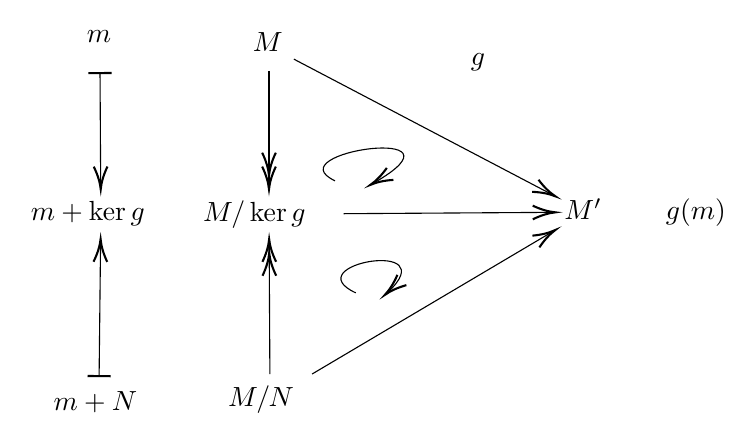
\begin{tikzpicture}[x=0.75pt,y=0.75pt,yscale=-1,xscale=1]
  %uncomment if require: \path (0,300); %set diagram left start at 0, and has height of 300

  %Curve Lines [id:da06639929221173313]
  \draw    (291.8,208.9) .. controls (262.25,195.11) and (335.54,182.29) .. (307.17,208.67) ;
  \draw [shift={(305.8,209.9)}, rotate = 318.81] [color={rgb, 255:red, 0; green, 0; blue, 0 }  ][line width=0.75]    (10.93,-3.29) .. controls (6.95,-1.4) and (3.31,-0.3) .. (0,0) .. controls (3.31,0.3) and (6.95,1.4) .. (10.93,3.29)   ;
  %Curve Lines [id:da2113069658179978]
  \draw    (281.8,154.9) .. controls (252.1,141.04) and (350.79,127.18) .. (300.37,156.01) ;
  \draw [shift={(298.8,156.9)}, rotate = 330.95] [color={rgb, 255:red, 0; green, 0; blue, 0 }  ][line width=0.75]    (10.93,-3.29) .. controls (6.95,-1.4) and (3.31,-0.3) .. (0,0) .. controls (3.31,0.3) and (6.95,1.4) .. (10.93,3.29)   ;

  % Text Node
  \draw (241,82.4) node [anchor=north west][inner sep=0.75pt]    {$M$};
  % Text Node
  \draw (391,162.4) node [anchor=north west][inner sep=0.75pt]    {$M'$};
  % Text Node
  \draw (346,92.4) node [anchor=north west][inner sep=0.75pt]    {$g$};
  % Text Node
  \draw (217,163.4) node [anchor=north west][inner sep=0.75pt]    {$M/\ker g$};
  % Text Node
  \draw (229,252.4) node [anchor=north west][inner sep=0.75pt]    {$M/N$};
  % Text Node
  \draw (145,255.4) node [anchor=north west][inner sep=0.75pt]    {$m+N$};
  % Text Node
  \draw (134,163.4) node [anchor=north west][inner sep=0.75pt]    {$m+\ker g$};
  % Text Node
  \draw (161,81.4) node [anchor=north west][inner sep=0.75pt]    {$m$};
  % Text Node
  \draw (440,162.4) node [anchor=north west][inner sep=0.75pt]    {$g( m)$};
  % Connection
  \draw    (262,96.3) -- (386.23,161.46) ;
  \draw [shift={(388,162.39)}, rotate = 207.68] [color={rgb, 255:red, 0; green, 0; blue, 0 }  ][line width=0.75]    (10.93,-3.29) .. controls (6.95,-1.4) and (3.31,-0.3) .. (0,0) .. controls (3.31,0.3) and (6.95,1.4) .. (10.93,3.29)   ;
  % Connection
  \draw    (250,102) -- (250,159) ;
  \draw [shift={(250,159)}, rotate = 270] [color={rgb, 255:red, 0; green, 0; blue, 0 }  ][line width=0.75]    (17.64,-3.29) .. controls (13.66,-1.4) and (10.02,-0.3) .. (6.71,0) .. controls (10.02,0.3) and (13.66,1.4) .. (17.64,3.29)(10.93,-3.29) .. controls (6.95,-1.4) and (3.31,-0.3) .. (0,0) .. controls (3.31,0.3) and (6.95,1.4) .. (10.93,3.29)   ;
  % Connection
  \draw    (250.43,248) -- (250.07,183) ;
  \draw [shift={(250.07,183)}, rotate = 449.68] [color={rgb, 255:red, 0; green, 0; blue, 0 }  ][line width=0.75]    (17.64,-3.29) .. controls (13.66,-1.4) and (10.02,-0.3) .. (6.71,0) .. controls (10.02,0.3) and (13.66,1.4) .. (17.64,3.29)(10.93,-3.29) .. controls (6.95,-1.4) and (3.31,-0.3) .. (0,0) .. controls (3.31,0.3) and (6.95,1.4) .. (10.93,3.29)   ;
  % Connection
  \draw    (270.77,248) -- (386.28,179.6) ;
  \draw [shift={(388,178.59)}, rotate = 509.37] [color={rgb, 255:red, 0; green, 0; blue, 0 }  ][line width=0.75]    (10.93,-3.29) .. controls (6.95,-1.4) and (3.31,-0.3) .. (0,0) .. controls (3.31,0.3) and (6.95,1.4) .. (10.93,3.29)   ;
  % Connection
  \draw    (286,170.76) -- (386,170.11) ;
  \draw [shift={(388,170.1)}, rotate = 539.62] [color={rgb, 255:red, 0; green, 0; blue, 0 }  ][line width=0.75]    (10.93,-3.29) .. controls (6.95,-1.4) and (3.31,-0.3) .. (0,0) .. controls (3.31,0.3) and (6.95,1.4) .. (10.93,3.29)   ;
  % Connection
  \draw    (168.15,249) -- (168.85,185) ;
  \draw [shift={(168.87,183)}, rotate = 450.62] [color={rgb, 255:red, 0; green, 0; blue, 0 }  ][line width=0.75]    (10.93,-3.29) .. controls (6.95,-1.4) and (3.31,-0.3) .. (0,0) .. controls (3.31,0.3) and (6.95,1.4) .. (10.93,3.29)   ;
  \draw [shift={(168.15,249)}, rotate = 450.62] [color={rgb, 255:red, 0; green, 0; blue, 0 }  ][line width=0.75]    (0,5.59) -- (0,-5.59)   ;
  % Connection
  \draw    (168.59,103) -- (168.91,157) ;
  \draw [shift={(168.93,159)}, rotate = 269.65] [color={rgb, 255:red, 0; green, 0; blue, 0 }  ][line width=0.75]    (10.93,-3.29) .. controls (6.95,-1.4) and (3.31,-0.3) .. (0,0) .. controls (3.31,0.3) and (6.95,1.4) .. (10.93,3.29)   ;
  \draw [shift={(168.59,103)}, rotate = 269.65] [color={rgb, 255:red, 0; green, 0; blue, 0 }  ][line width=0.75]    (0,5.59) -- (0,-5.59)   ;

  \end{tikzpicture}
\end{remark}

\begin{proposition} Dados dos $A$-módulos $M$ y $N$, existe un $A$-módulo $M\otimes_AN$ y una aplicación $A$-bilineal $\delta:M\times N\rightarrow M\otimes_AN$ tal que para cada $A$-módulo $P$ y para cada $F:M\times N\rightarrow P$ $A$-bilineal, existe una única aplicación $A$-lineal $f:M\otimes_AN:\rightarrow P$ tal que $f\circ\delta =F$.

Además, el par $(\delta,M\otimes_AN)$ es único, en el sentido que de existir otro par $(\delta',T)$ que verifique las condiciones del enunciado, se tiene que $T\cong M\otimes_AN$.
\end{proposition}
\begin{proof}
Para ver la unicidad, supongamos que $(\delta,T)$ y $(\delta',T')$  cumplen las condiciones de la proposición. Poniendo a $T'$ como $P$ y a $\delta'$ como $F$, el resultado garantiza la existencia de $j:T\rightarrow T'$ tal que $\delta'=j\circ\delta$. Intercambiando los roles de $T$ y $T'$, se tiene $j':T'\rightarrow T$ tal que $\delta=j'\circ\delta'$. Entonces, cada una de las composiciones $j\circ j'$ y $j'\circ j$ son la identidad, lo cual garantiza que $j$ sea un isomorfismo.

Para la existencia, procedemos como sigue. Consideremos $A^{(M\times N)}$, la suma directa de $A$ tantas veces como elementos tenga $M\times N$. Definimos el siguiente subconjunto de $A^{(M\times N)}$
\begin{multline}
  S=\{e_{(m+m',n)}-e_{(m,n)}-e_{(m',n)}, e_{(m,n+n')}-e_{(m,n)}-e_{(m,n')}, \\ e_{(m,\lambda n)}-\lambda e_{(m,n)}, e_{(\lambda m,n)}-\lambda e_{(m,n)}\}
\end{multline}
con $m,m'\in M$, $n,n'\in N$ y $\lambda\in A$.

Ahora tomamos $\Sigma$ el submódulo generado por $S$. Se cumple $\Sigma\subset A^{(M\times N)}$, luego podemos definir el cociente $A^{(M\times N)}/\Sigma$, que es un $A$-módulo:
$$\begin{array}{rcl}
    M\times N&\overset{\delta}{\longrightarrow}&M\otimes_A N:=\faktor{A^{(M\times N)}}{\Sigma}\\
    (m,n)&\longmapsto&[e_{(m,n)}]
    \end{array}$$
La aplicación $\delta$ es bilineal por construcción. Además, $\{[e_{(m,n)}]: (m,n)\in M\times N\}$ es un sistema de generadores de $M\otimes_A N$.

Cada aplicación $f:M\times N \to P$ se extiende por linealidad a un homomorfismo de $A$-módulos $f:A^{(M\times N)} \to P$, tomando $f(e_{(m,n)}) = f(m,n)$, $f(e_{(m,n)}+e_{(m,n)}) = f(m,n)+f(m',n')$, y $f(\lambda e_{(m,n)}) = \lambda f(m,n)$. En particular, dada $F:M\times N \to P$ es bilineal, definimos el homomorfismo de $A$-módulos
$$\begin{array}{rrcl}
	f_0:&A^{M\times N}&\longrightarrow&P  \\
	&e_{(m,n)}&\longmapsto&F(m,n)
	\end{array}$$

Para poder pasar al cociente solo hemos de comprobar que $\Sigma\subset ker(f_0)$. Como $\Sigma$ está generado por $S$, basta ver $S\subset ker(f_0)$. Pero esto es directo por ser $F$ bilineal y la definición de $S$. Por ejemplo, $$f_0(e_{(m+m',n)}-e_{(m,n)}-e_{(m',n)})=F(e_{(m+m',n)}-e_{(m,n)}-e_{(m',n)})=0$$. Así, la siguiente aplicación está bien definida y cumple las condiciones del teorema
$$\begin{array}{rrcl}
	\tilde{f_0}:&\faktor{A^{M\times N}}{\Sigma}&\longrightarrow&P  \\
	&[e_{(m,n)}]&\longmapsto&F(m,n)
	\end{array}$$
\end{proof}

\begin{definition}
  Al $A$-módulo $M\otimes N$ se le llama \emph{producto tensorial} de $M$ y $N$.
\end{definition}

\begin{remark}
  Observamos que la construcción es de lo más natural. Otra forma de escribir la construcción es pensar que hemos tomado todos los elementos del producto cartesiano de la forma $(m+m',n)-(m,n)-(m',n), (m,n+n') - (m,n)-(m,n'),  (m,\lambda n) -\lambda (m,n), \lambda (m,n) -\lambda (m,n)$, es decir, hemos seleccionado unas relaciones que queremos que se cumplan (de bilinealidad). Al cocientar por el módulo que generan, estamos imponiendo que cada uno de esos elementos sea 0, que $[(m+m',n)]= [(m,n)]+[(m',n)]$, etc.
\end{remark}

\begin{remark}
De ahora en adelante omitiremos el subíndice de $\otimes_A$, escribiendo $M \otimes N$ siempre que no de lugar a confusión. Entonces
\begin{enumerate}
  \item A las clases $[e_{(m,n)}]$ se les denota $m\otimes n$.

  Todo elemento de $M\otimes N$ es suma $\sum_{i=1}^rm_j\otimes n_j$, para ciertos $m_j\in M$, $n_j\in N$ y $r\in\mathbb{N}$, ya que $[\lambda e_{(m,n)}]=[e_{(\lambda m,n)}]=[e_{(m,\lambda n)}]$ por la definición inicial de $S$.

  \item Las aplicaciones bilineales de $M\times N$ en $P$, $\Bil_A(M\times N,P)$ están en correspondencia biyectiva con $\Hom_A(M\otimes N,P)$.

  En particular, si tomamos $A$ como $K$ cuerpo y $M$ y $N$ $K$-espacios vectoriales,$$\Hom_A(M\otimes_KN,K)=(M\otimes_KN)^{\ast}=\Bil_K(M\times N,K)$$

  \item La construcción del producto tensorial de módulos se puede generalizar. Dados unos $A$-módulos $M_1,\dots,M_r$, existe un $A$-módulo $M_1\otimes \dots\otimes M_r$ y $\delta:M_1\times\dots\times,M_r\longrightarrow M_1\otimes \dots\otimes M_r$ multilineal tal que para cualquier aplicación $A$-multilineal $\Phi:M_1\times\dots\times,M_r\longrightarrow P$, existe una única $f:M_1\otimes \dots\otimes M_r\longrightarrow P$ $A$-lineal tal que $f\circ\delta=F$

\end{enumerate}
\end{remark}

\begin{lemma} \label{generadores} Sean $Z$ y $Z'$ dos $A$-módulos. Sea $\{z_i\}_{i\in I}$ un sistema de generadores de $Z$ y sea $\{z_j'\}_{j\in J}$ un sistema de generadores de $Z'$. Entonces, $\{z_i\otimes z_j:(i,j)\in I\times J\}$ es un sistema de generadores de $Z\otimes Z'$.
\end{lemma}
\begin{proposition} Sea $A$ un anillo conmutativo unitario. Se cumple:\begin{enumerate}
    \item Dados $M,N$ y $P$ $A$-módulos, $$M\otimes N\otimes P\cong(M\otimes N)\otimes P$$
    \item $M\otimes N=N\otimes M$
    \item Dados $f:M_1\rightarrow M_2$ y $g:N_1\rightarrow N_2$ $A$-lineales, existe $f\otimes g:M_1\otimes N_1\rightarrow M_2\otimes N_2$ $A$-lineal tal que si tenemos $f':M_2\rightarrow M_3$ y $g':N_2\rightarrow N_3$ homomorfismos de $A$-módulos, $$M_1\otimes N_1\overset{f\otimes g}{\longrightarrow} M_2\otimes N_2\overset{f'\otimes g'}{\longrightarrow} M_3\otimes N_3$$ se cumple $$(f'\otimes g')\circ(f\otimes g)=(f'\circ f)\otimes (g'\circ g)$$
    \item Si $B$ es un $A$-álgebra, $B\otimes M$ es un $B$-módulo
    \item Si $B$ y $C$ son $A$-álgebras, $B\otimes C$ es un $A$-álgebra, un $B$-módulo y un $C$-módulo
    \item Para todo $P$ $A$-módulo, se verifica $P\otimes_A A\cong P$ mediante el siguiente isomorfismo de $A$-módulos
    $$\begin{array}{rcl}
    P&\longrightarrow&P\otimes_A A  \\
    p&\longmapsto&p\otimes_A 1_A
    \end{array}$$
    \item Sean ${\set {N_i}}_{i\in I}$ y $M$ $A$-módulos. Se cumple que $$M\otimes_A\left(\bigoplus_{i\in I}N_i\right)\cong\bigoplus_{i\in I}(M\otimes_A N_i).$$
    En particular,
    $$M\otimes_A A^{(I)}\cong\bigoplus_{i\in I}(M\otimes_A A)\cong M^{(I)}.$$
    \end{enumerate}
\end{proposition}
\begin{proof}
Comprobamos cada cosa.

\textit{1.} Definimos la aplicación $A$-trilineal
$$ \begin{array}{rrcl}
     F:&M\times N\times P&\longrightarrow&(M\otimes N)\otimes P\\
     &(m,n,p)&\longmapsto&(m\otimes n)\otimes p
\end{array}
$$
Existe una única $f:M\otimes N\otimes P\rightarrow (M\otimes N)\otimes P$ tal que $f(m\otimes n\otimes p)=F(m,n,p)=(m\otimes n)\otimes p$,

\begin{figure}[h!]
  \centering

  \tikzset{every picture/.style={line width=0.75pt}} %set default line width to 0.75pt

  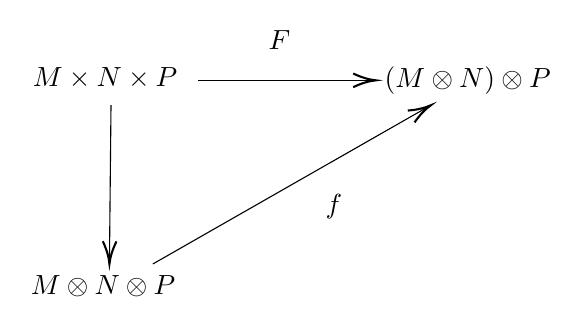
\begin{tikzpicture}[x=0.75pt,y=0.75pt,yscale=-1,xscale=1]
  %uncomment if require: \path (0,300); %set diagram left start at 0, and has height of 300


  % Text Node
  \draw (178.2,82.9) node [anchor=north west][inner sep=0.75pt]    {$M\times N\times P$};
  % Text Node
  \draw (347.7,82.9) node [anchor=north west][inner sep=0.75pt]    {$( M\otimes N) \otimes P$};
  % Text Node
  \draw (177.2,183.4) node [anchor=north west][inner sep=0.75pt]    {$M\otimes N\otimes P$};
  % Text Node
  \draw (291.7,65.4) node [anchor=north west][inner sep=0.75pt]    {$F$};
  % Text Node
  \draw (319.2,143.9) node [anchor=north west][inner sep=0.75pt]    {$f$};
  % Connection
  \draw    (259.2,90.5) -- (342.7,90.5) ;
  \draw [shift={(344.7,90.5)}, rotate = 180] [color={rgb, 255:red, 0; green, 0; blue, 0 }  ][line width=0.75]    (10.93,-3.29) .. controls (6.95,-1.4) and (3.31,-0.3) .. (0,0) .. controls (3.31,0.3) and (6.95,1.4) .. (10.93,3.29)   ;
  % Connection
  \draw    (217.08,102.5) -- (216.34,177) ;
  \draw [shift={(216.32,179)}, rotate = 270.57] [color={rgb, 255:red, 0; green, 0; blue, 0 }  ][line width=0.75]    (10.93,-3.29) .. controls (6.95,-1.4) and (3.31,-0.3) .. (0,0) .. controls (3.31,0.3) and (6.95,1.4) .. (10.93,3.29)   ;
  % Connection
  \draw    (237.21,179) -- (369.45,103.49) ;
  \draw [shift={(371.19,102.5)}, rotate = 510.27] [color={rgb, 255:red, 0; green, 0; blue, 0 }  ][line width=0.75]    (10.93,-3.29) .. controls (6.95,-1.4) and (3.31,-0.3) .. (0,0) .. controls (3.31,0.3) and (6.95,1.4) .. (10.93,3.29)   ;

  \end{tikzpicture}
\end{figure}

Veamos como definir la flecha en sentido contrario. Para cada $p\in P$ definimos la aplicación $A$-bilineal
$$\begin{array}{rrcl}
	\Phi_p:&M\times N&\longrightarrow&M\otimes N\otimes P  \\
	&(m,n)&\longmapsto&m\otimes n\otimes p
	\end{array}$$
Existe una única $\varphi_p:M\otimes N\rightarrow M\otimes N\otimes P$ tal que $\varphi_p(m\otimes n)=\Phi_p(m,n)=m\otimes n\otimes p$

\begin{figure}[h!]
  \centering

  \tikzset{every picture/.style={line width=0.75pt}} %set default line width to 0.75pt

  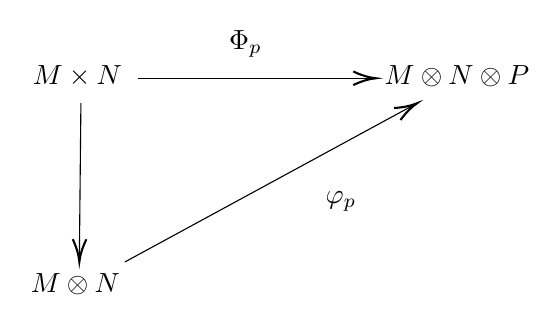
\begin{tikzpicture}[x=0.75pt,y=0.75pt,yscale=-1,xscale=1]
  %uncomment if require: \path (0,300); %set diagram left start at 0, and has height of 300


  % Text Node
  \draw (178.2,82.9) node [anchor=north west][inner sep=0.75pt]    {$M\times N$};
  % Text Node
  \draw (347.7,82.9) node [anchor=north west][inner sep=0.75pt]    {$M\otimes N\otimes P$};
  % Text Node
  \draw (177.2,183.4) node [anchor=north west][inner sep=0.75pt]    {$M\otimes N$};
  % Text Node
  \draw (272.7,66.4) node [anchor=north west][inner sep=0.75pt]    {$\Phi _{p}$};
  % Text Node
  \draw (319.2,143.9) node [anchor=north west][inner sep=0.75pt]    {$\varphi _{p}$};
  % Connection
  \draw    (230.2,90.5) -- (342.7,90.5) ;
  \draw [shift={(344.7,90.5)}, rotate = 180] [color={rgb, 255:red, 0; green, 0; blue, 0 }  ][line width=0.75]    (10.93,-3.29) .. controls (6.95,-1.4) and (3.31,-0.3) .. (0,0) .. controls (3.31,0.3) and (6.95,1.4) .. (10.93,3.29)   ;
  % Connection
  \draw    (202.58,102.5) -- (201.84,177) ;
  \draw [shift={(201.82,179)}, rotate = 270.57] [color={rgb, 255:red, 0; green, 0; blue, 0 }  ][line width=0.75]    (10.93,-3.29) .. controls (6.95,-1.4) and (3.31,-0.3) .. (0,0) .. controls (3.31,0.3) and (6.95,1.4) .. (10.93,3.29)   ;
  % Connection
  \draw    (223.79,179) -- (362.85,103.45) ;
  \draw [shift={(364.61,102.5)}, rotate = 511.49] [color={rgb, 255:red, 0; green, 0; blue, 0 }  ][line width=0.75]    (10.93,-3.29) .. controls (6.95,-1.4) and (3.31,-0.3) .. (0,0) .. controls (3.31,0.3) and (6.95,1.4) .. (10.93,3.29)   ;

  \end{tikzpicture}
\end{figure}

Observamos que si $p,p'\in P$, entonces $\varphi_p + \varphi_{p'}=\varphi_{p+p'}$ por unicidad ya que ambas completan el diagrama: $\varphi_p(m\otimes n)+\varphi_{p'}(m\otimes n) = m\otimes n\otimes p + m\otimes n\otimes p' = m\otimes n\otimes (p+p') = \varphi_{p+p'}(m\otimes n)$. Lo mismo ocurre con $\lambda \varphi_p = \varphi_{\lambda p}$.

Sea entonces la aplicación $A$-bilineal
$$\begin{array}{rrcl}
	G:&(M\otimes N)\times P&\longrightarrow&M\otimes N\otimes P  \\
	&(z,p)&\longmapsto&\varphi_p(z)
	\end{array}$$
Existe una única $g:(M\otimes N)\otimes P\rightarrow M\otimes N\otimes P$ aplicación $A$-lineal que hace conmutativo el diagrama siguiente

\begin{figure}[h!]
  \centering
  \tikzset{every picture/.style={line width=0.75pt}} %set default line width to 0.75pt

  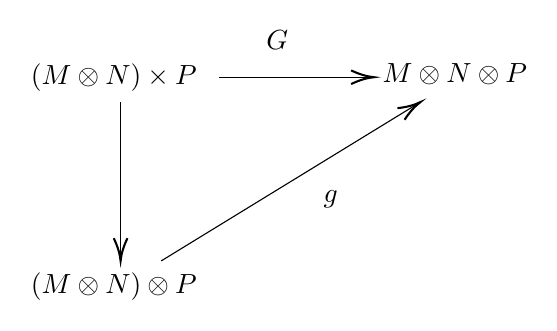
\begin{tikzpicture}[x=0.75pt,y=0.75pt,yscale=-1,xscale=1]
  %uncomment if require: \path (0,300); %set diagram left start at 0, and has height of 300


  % Text Node
  \draw (178.2,82.9) node [anchor=north west][inner sep=0.75pt]    {$( M\otimes N) \times P$};
  % Text Node
  \draw (347.7,82.9) node [anchor=north west][inner sep=0.75pt]    {$M\otimes N\otimes P$};
  % Text Node
  \draw (178.2,183.4) node [anchor=north west][inner sep=0.75pt]    {$( M\otimes N) \otimes P$};
  % Text Node
  \draw (291.7,66.9) node [anchor=north west][inner sep=0.75pt]    {$G$};
  % Text Node
  \draw (319.2,143.9) node [anchor=north west][inner sep=0.75pt]    {$g$};
  % Connection
  \draw    (270.2,90.5) -- (342.7,90.5) ;
  \draw [shift={(344.7,90.5)}, rotate = 180] [color={rgb, 255:red, 0; green, 0; blue, 0 }  ][line width=0.75]    (10.93,-3.29) .. controls (6.95,-1.4) and (3.31,-0.3) .. (0,0) .. controls (3.31,0.3) and (6.95,1.4) .. (10.93,3.29)   ;
  % Connection
  \draw    (222.7,102.5) -- (222.7,177) ;
  \draw [shift={(222.7,179)}, rotate = 270] [color={rgb, 255:red, 0; green, 0; blue, 0 }  ][line width=0.75]    (10.93,-3.29) .. controls (6.95,-1.4) and (3.31,-0.3) .. (0,0) .. controls (3.31,0.3) and (6.95,1.4) .. (10.93,3.29)   ;
  % Connection
  \draw    (242.28,179) -- (365.41,103.55) ;
  \draw [shift={(367.12,102.5)}, rotate = 508.5] [color={rgb, 255:red, 0; green, 0; blue, 0 }  ][line width=0.75]    (10.93,-3.29) .. controls (6.95,-1.4) and (3.31,-0.3) .. (0,0) .. controls (3.31,0.3) and (6.95,1.4) .. (10.93,3.29)   ;

  \end{tikzpicture}
\end{figure}

Veamos entonces que la composición de ambas es la identidad. Para ello solo hace falta ver que deja los generadores de cada $A$-módulo invariantes. Efectivamente,

\begin{align*}
  M\otimes N \otimes P &\overset{f}{\longrightarrow}(M\otimes N )\otimes P \overset{g}{\longrightarrow}M\otimes N \otimes P\\
  m\otimes n\otimes p &\longmapsto (m\otimes n)\otimes p \longmapsto m\otimes n\otimes p
\end{align*}

Por tanto, $g\circ f=Id_{M\otimes N\otimes P}$

Por otro, $\{m\otimes n:(m,n)\in M\times N\}$ es sistema de generadores de $M\otimes N$. Por el lema \ref{generadores}, $\{(m\otimes n)\otimes p: (m,n,p)\in M\times N\times P\}$ es sistema de generadores de $(M\otimes N)\otimes P$. Evaluando, $(f\circ g)((m\otimes n)\otimes p)=(m\otimes n)\otimes p)$ y concluimos $f\circ g)=Id_{(M\otimes N)\otimes P}$.

\textit{2.} Siguiendo el esquema de \textit{1}, solo hay que definir las aplicaciones naturales $M\times N \to N\otimes M$ que llevan $(m,n)\mapsto n\otimes m$ y la análoga en la otra dirección, que pasan al producto tensorial, y cuya composición resulta en la identidad. Para comprobar esto último solo hay que verlo para los generadores que es trivial.

\textit{3.} Definimos la aplicación $A$-bilineal $M_1\times N_1 \to M_2\times N_2$ dada por $(m_1,n_1) \mapsto f(m_1)\otimes g(n_1)$. Entonces existe una única $M_1\otimes N_1 \to M_2 \otimes N_2$ lineal que completa el diagrama conmutativo habitual.

Lo mismo sucede con $M_2\times N_2 \to M_3\times N_3$, de forma que obtenemos el diagrama

\begin{figure}[h!]
  \centering


  \tikzset{every picture/.style={line width=0.75pt}} %set default line width to 0.75pt

  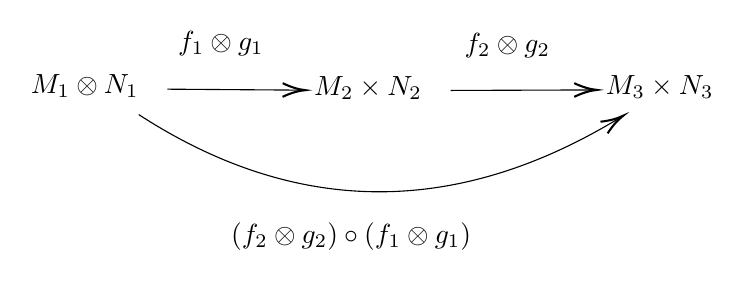
\begin{tikzpicture}[x=0.75pt,y=0.75pt,yscale=-1,xscale=1]
  %uncomment if require: \path (0,300); %set diagram left start at 0, and has height of 300


  % Text Node
  \draw (311.2,61.9) node [anchor=north west][inner sep=0.75pt]    {$M_{2} \times N_{2}$};
  % Text Node
  \draw (174.7,60.9) node [anchor=north west][inner sep=0.75pt]    {$M_{1} \otimes N_{1}$};
  % Text Node
  \draw (245.7,39.9) node [anchor=north west][inner sep=0.75pt]    {$f_{1} \otimes g_{1}$};
  % Text Node
  \draw (383.7,40.9) node [anchor=north west][inner sep=0.75pt]    {$f_{2} \otimes g_{2}$};
  % Text Node
  \draw (451.7,61.4) node [anchor=north west][inner sep=0.75pt]    {$M_{3} \times N_{3}$};
  % Text Node
  \draw (271.2,132.4) node [anchor=north west][inner sep=0.75pt]    {$( f_{2} \otimes g_{2}) \circ ( f_{1} \otimes g_{1})$};
  % Connection
  \draw    (241.7,69.26) -- (306.2,69.73) ;
  \draw [shift={(308.2,69.74)}, rotate = 180.42] [color={rgb, 255:red, 0; green, 0; blue, 0 }  ][line width=0.75]    (10.93,-3.29) .. controls (6.95,-1.4) and (3.31,-0.3) .. (0,0) .. controls (3.31,0.3) and (6.95,1.4) .. (10.93,3.29)   ;
  % Connection
  \draw    (378.2,69.88) -- (446.7,69.63) ;
  \draw [shift={(448.7,69.62)}, rotate = 539.8] [color={rgb, 255:red, 0; green, 0; blue, 0 }  ][line width=0.75]    (10.93,-3.29) .. controls (6.95,-1.4) and (3.31,-0.3) .. (0,0) .. controls (3.31,0.3) and (6.95,1.4) .. (10.93,3.29)   ;
  % Connection
  \draw    (227.94,81.5) .. controls (303.73,130.68) and (381.17,131.1) .. (460.25,82.73) ;
  \draw [shift={(461.44,82)}, rotate = 508.3] [color={rgb, 255:red, 0; green, 0; blue, 0 }  ][line width=0.75]    (10.93,-3.29) .. controls (6.95,-1.4) and (3.31,-0.3) .. (0,0) .. controls (3.31,0.3) and (6.95,1.4) .. (10.93,3.29)   ;

  \end{tikzpicture}
\end{figure}

Podemos definir la aplicación $A$-bilineal $M_1\times N_1 \to M_3 \otimes N_3$ dada por $(m_1,n_1)\mapsto(f_2\circ f_1)(m_1)\otimes (g_2\circ g_1)(n_1)$, y así existe una única aplicación $M_1\otimes N_1 \to M_3 \otimes N_3$ que cierra el diagrama conmutativo, y por unicidad ha de coincidir con la composición de arriba.

\textit{4.} Queremos definir un producto externo. Empezamos definiendo para cada $b\in B$ la aplicación $A$-lineal $\Phi_b:B\times M \to  B\otimes M$ dada por $(b',m)\mapsto bb'\otimes m$. Entonces existe una única aplicación lineal del producto tensorial que cierra el diagrama

\begin{figure}[h!]
  \centering

  \tikzset{every picture/.style={line width=0.75pt}} %set default line width to 0.75pt

  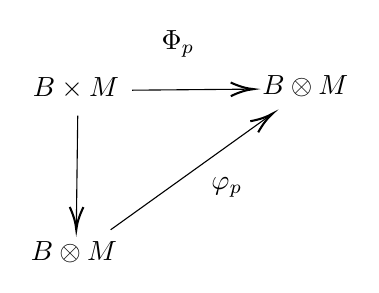
\begin{tikzpicture}[x=0.75pt,y=0.75pt,yscale=-1,xscale=1]
  %uncomment if require: \path (0,300); %set diagram left start at 0, and has height of 300


  % Text Node
  \draw (201.2,63.4) node [anchor=north west][inner sep=0.75pt]    {$B\times M$};
  % Text Node
  \draw (311.7,62.4) node [anchor=north west][inner sep=0.75pt]    {$B\otimes M$};
  % Text Node
  \draw (200.2,142.4) node [anchor=north west][inner sep=0.75pt]    {$B\otimes M$};
  % Text Node
  \draw (263.2,40.9) node [anchor=north west][inner sep=0.75pt]    {$\Phi _{p}$};
  % Text Node
  \draw (287.2,111.4) node [anchor=north west][inner sep=0.75pt]    {$\varphi _{p}$};
  % Connection
  \draw    (224.05,83) -- (223.38,136) ;
  \draw [shift={(223.35,138)}, rotate = 270.73] [color={rgb, 255:red, 0; green, 0; blue, 0 }  ][line width=0.75]    (10.93,-3.29) .. controls (6.95,-1.4) and (3.31,-0.3) .. (0,0) .. controls (3.31,0.3) and (6.95,1.4) .. (10.93,3.29)   ;
  % Connection
  \draw    (250.2,70.76) -- (306.7,70.25) ;
  \draw [shift={(308.7,70.24)}, rotate = 539.48] [color={rgb, 255:red, 0; green, 0; blue, 0 }  ][line width=0.75]    (10.93,-3.29) .. controls (6.95,-1.4) and (3.31,-0.3) .. (0,0) .. controls (3.31,0.3) and (6.95,1.4) .. (10.93,3.29)   ;
  % Connection
  \draw    (239.92,138) -- (316.35,83.17) ;
  \draw [shift={(317.97,82)}, rotate = 504.34] [color={rgb, 255:red, 0; green, 0; blue, 0 }  ][line width=0.75]    (10.93,-3.29) .. controls (6.95,-1.4) and (3.31,-0.3) .. (0,0) .. controls (3.31,0.3) and (6.95,1.4) .. (10.93,3.29)   ;

  \end{tikzpicture}
\end{figure}

Se cumple que $\varphi_{b_1+b_2} = \varphi_{b_1}+\varphi_{b_2}$ y que $\varphi_{b_1b_2} = \varphi_{b_1}\circ\varphi_{b_2}$ por la unicidad. De esta forma podemos definir la aplicación

\begin{align}
  \Phi: B\times(B\otimes M) &\to B\otimes M\\
  (b,z) &\mapsto \varphi_b(z)
\end{align}
que está bien definida y con la cual $B\otimes M$ cumple los axiomas de $A$-módulo.

\textit{7.} Denotemos por $n_i\in \oplus_{i\in I}N_i$ al elemento tal que tiene a $n\in N_i$ por $i$-ésima coordenada y $0$ en el resto. Definamos la aplicación
$$\begin{array}{rrcl}
F:&M\times(\oplus_{i\in I})&\longrightarrow&\oplus_{i\in I}(M\otimes_A N_i)\\
&(m,n_i)&\longmapsto& (m\otimes n)_i
\end{array}.$$
Esta aplicación es bilineal por serlo para el sistema de generadores
\begin{align*}
F(\lambda m,n_i)=(\lambda m\otimes n)_i=&(m\otimes \lambda n)_i=F(m,\lambda n)\\
=&\lambda(m\otimes n)_i=\lambda F(m,n_i),\\
F(m_1+m_2,n_i)=&((m_1+m_2)\otimes n)_i=\\=&(m_1\otimes n)_i+(m_2\otimes n)_i=F(m_1,n_i)+F(m_2,n_i)\hspace{10pt}\text{y}\\
F(m,(n_1+n_2)_i)=&(m\otimes(n_1+n_2))_i=\\=&(m\otimes n_1)_i+(m\otimes n_2)_i=F(m,{n_1}_i)+F(m,{n_2}_i).
\end{align*}
Es por esto que existe
$$\begin{array}{rrcl}
f:&M\otimes_A(\oplus_{i\in I}N_i)&\longrightarrow&\oplus_{i\in I}(M\otimes_A N_i)
\end{array}$$
aplicación $A$-lineal. En el otro sentido comenzamos definiendo para cada $i\in I$ las aplicaciones
$$\begin{array}{rrcl}
G_i:&M\times N_i&\longmapsto&M\otimes(\oplus_{i\in I}N_i)\\
&(m,n)&\longmapsto&m\otimes n_i
\end{array},$$
que son $A$-bilineales de nuevo por la propia definición. Así, surgen las apliciones $A$-lineales
$$\begin{array}{rrcl}
g_i&M\otimes N_i&\longrightarrow&M\otimes(\oplus_{i\in I}N_i)
\end{array},$$
que nos permiten definir a su vez la siguiente aplicación $A$-lineal
$$\begin{array}{rrcl}
g:=\oplus_{i\in I}g_i:&\oplus(M\otimes_A N_i)&\longrightarrow&M\otimes_A(\oplus_{i\in I}N_i)  \\
&
\end{array}.$$
Se comprueba que $g\circ f=1_{M\otimes_A(\oplus N_i)}$ y $f\circ g=1_{\oplus(M\otimes_A N_i)}$ y se tiene el resultado.

Para ver el caso particular, basta aplicar lo que acabamos de probar y la propiedad $6$ del producto tensorial.

\end{proof}


En estas construcciones se tienen las siguientes propiedades.
\begin{itemize}
    \item [1)] Dados $M_1,M_2$ y $M_3$ $A$-módulos, $M_1\otimes  M_2\otimes M_3\cong(M_1\otimes  M_2)\otimes  M_3\cong M_1\otimes (M_2\otimes  M_3)$
    \item [2)] $M\otimes N=N\otimes M$
    \item [3)] Dados $f:M_1'\to M_1$ y $g:M_2'\to M_2$ $A$-lineales, existe $f\otimes g:M_1'\otimes  M_2'\rightarrow M_1\otimes M_2$ $A$-lineal tal que el diagrama es conmutativo.

    En particular, si $M\in Obj(Mod_A)$, $M\otimes\_$ es un funtor covariante de $Mod_A$ en $Mod_A$ (Véase Apéndice A)
\end{itemize}

Ahora, dado un $A$-módulo $M$, consideremos el funtor
$$\begin{array}{rcl}
Mod_A&\overset{M\oplus_A\_}{\longrightarrow}&Mod_A\\
N&\longmapsto&M\oplus_A N
\end{array}$$
y estudiemos su comportamiento respecto de sucesiones exactas. Antes de comenzar, cabe destacar que estudiar este funtor es equivalente a estudiar el funtor $\_\oplus_A M$ debido al isomorfismo existente $M\oplus_A N\cong N\oplus_A M$.

\begin{proposition}
	Sea $M$ un $A$-módulo y sea \begin{equation}\label{equation: ext1}
	N'\overset{f}{\longrightarrow}N\overset{g}{\longrightarrow}N''\longrightarrow 0
	\end{equation}una sucesión exacta. Se cumple que \begin{equation}\label{equation: ext2}
	M\otimes_A N'\overset{1_M\otimes f}{\longrightarrow}M\otimes_A N\overset{1_M\otimes g}{\longrightarrow}M\otimes_A N''\longrightarrow 0
	\end{equation} es también una sucesión exacta.
\end{proposition}

\begin{proof}
	Sabemos que ($\ref{equation: ext1}$) es exacta si, y sólo si, para todo $P$ $A$-módulo se tiene que la sucesión
	\begin{equation}\label{equation: ext3}
	0\longrightarrow\Hom_A(M\oplus_A N'',P)\overset{(1_M\oplus g)^*}{\longrightarrow}\Hom_A(M\oplus_A N,P)\overset{(1_M\oplus f)^*}{\longrightarrow}\Hom_A(M\oplus_A N',P)
	\end{equation}
	es exacta.

	La sucesión
	\begin{align*}\label{equation: ext4}
	0\longrightarrow\Hom_A(M,\Hom_A(N,P))\overset{(g^{*_P})_{*_M}}{\longrightarrow}&\Hom_A(M,\Hom_A(N,P))\overset{(f^{*_P})_{*_M}}{\longrightarrow}\\
	\overset{(f^{*_P})_{*_M}}{\longrightarrow}&\Hom_A(M,\Hom_A(N,P)),
	\end{align*}
	donde $(f^{*_P})_{*_M}:=\Hom_A(M,\Hom_A(f,P))$ y $(g^{*_P})_{*_M}:=\Hom_A(M,\Hom_A(g,P))$, surge de aplicar en primer lugar el funtor $\Hom_A(\_,P)$ a la sucesión $\ref{equation: ext1}$ y, después, aplicar el funtor $\Hom_A(M,\_)$ al resultado anterior. Así, $\ref{pry}$ nos dice que es exacta.

	Observemos ahora que, para cada $X\in\set{N,N',N''}$ se tiene la cadena de isomorfismos de $A$-módulos
	$$\Hom_A(M\otimes_A X,P)\cong\Bil_A(M\times X,P)\cong\Hom_A(M,\Hom_A(X,P)).$$
	El primero de los isomorfismos es inmediato atendiendo a la propia definición del producto tensorial: Dada $F\in\Bil_A(M\times X,P)$, existe una única $\Bar{F}\in\Hom_A(M\otimes X,P)$ de forma que para cada par $(m,x)\in M\times X$ se verifica $\Bar{F}(m\otimes_A x)=F(m,x)$. Comprobemos el segundo de los isomorfismos. En primer lugar, definamos
	$$\begin{array}{rcl}
	\Bil_A(M\times X,P)&\longrightarrow&\Hom_A(M,\Hom_A(X,P))\\
	F(m,n)&\longmapsto&(\varphi_F(m))(n):=F(m,n)
	\end{array}.$$
	Dados $F,G\in\Bil_A(M\times X,P)$ y $\lambda\in A$ tenemos
	\begin{itemize}
		\item $(F+G)(n,m)=F(m,n)+G(m,n)$ y
		\item $(\lambda F)(m,n)=\lambda F(m,n).$
	\end{itemize}

	Por otro lado, definamos
	$$\begin{array}{rcl}
	\Hom_A(M,\Hom_A(X,P))&\longrightarrow&\Bil_A(M\times X,P)\\
	\varphi(m)(n)&\longmapsto&F_\varphi(m,n):=\varphi(m)(n)
	\end{array}.$$

	Veamos que la aplicación es bilienal. Sean $\varphi\in\Hom_A(M,\Hom_A(X,P))$, $\set{m,m_1,m_2}\subset M$, $\set{n,n_1,n_2}\subset X$ y $\lambda\in A$. Tenemos
	\begin{itemize}
		\item $\varphi(m_1+m_2)(n)=(\varphi(m_1)+\varphi(m_2))(n)=\varphi(m_1)(n)+\varphi(m_2)(n)$,
		\item $\varphi(m)(n_1+n_2)=\varphi(m)(n_1)+\varphi(m)(n_2)$ y
		\item $\varphi(\lambda m)(n)=(\lambda\varphi)(m)(n)=\lambda \varphi(m)(n)=\varphi(m)(\lambda n)$.
	\end{itemize}
	Vemos así que ambas aplicaciones son $A$-lineales. Por último, sean $F\in\Bil_A(M\times X,P)$ y $\varphi\in\Hom_A(M,\Hom_A(X,P))$ y veamos que la una es la inversa de la otra. Se tiene
	\begin{itemize}
		\item $\varphi_{F_\varphi}(m)(n)=F_\varphi(m,n)=\varphi(m)(n)$ y
		\item $F_{\varphi_F}(m,n)=\varphi_F(m)(n)=F(m,n).$
	\end{itemize}

	Denotemos $\Phi_X:\Hom_A(M\otimes_A X,P)\longrightarrow\Hom_A(M,\Hom_A(X,P))$, para cada $X\in\{N,N',N''\}$, a cada uno de los isomorfismos definidos.
	Estos isomorfismos implican que por ser ($\ref{equation: ext4}$) exacta ($\ref{equation: ext3}$) es también exacta. Para probar esto es suficiente ver que se tienen las igualdades
	$$(1_M\otimes g)^*={\Phi_N}^{-1}\circ(g^*)_*\circ\Phi_{N''}$$
	y
	$$(1_M\otimes f)^*={\Phi_N'}^{-1}\circ(f^*)_*\circ\Phi_{N}.$$
	Probemos la primera de las igualdades. Dado $F\in\Hom_A(M\oplus N'',P)$, $\Phi_{N''}(F):=\varphi_F\in\Hom_A(M,\Hom_A(N'',P))$ y $$(g^*)_*(\varphi_F(m)(n))=g^*(\varphi_F(m))(n)=\varphi_F(m)(g(n))$$
	para cada $m\oplus n\in M\oplus_A N$. Por último,
	$${\Phi_N}^{-1}(\varphi_F(m)(g(n)))=F(m\oplus g(n))$$
	y
	$$F(m\oplus g(n))=F((1_M\oplus g)(m\oplus n)).$$
	Dado que $m\oplus n\in M\oplus_A N''$ era arbitrario, tenemos la igualdad que buscábamos.
	El caso de la $f$ es análogo.
\end{proof}

\begin{definition}
	Se dice que un $A$-módulo $M$ es plano si, y sólo si, el funtor $M\otimes_A \_$ es exacto, i.e, conserva sucesiones exactas.
\end{definition}

Antes de continuar con la siguiente proposición, observemos lo siguiente: dados $M,N$ $A$-módulos y $N'\subset N$ submódulo, un elemento $m\otimes_A n'\in M\otimes_A N'$ puede considerarse como un elemento en $M\otimes_A N'$ y como un elemento en $M\otimes_A N$ haciendo uso de la inclusión $$M\otimes_A N'\overset{i}{\hookrightarrow}M\otimes_A N;$$
sin embargo, de la pertenencia $m\otimes_A n'\in M\otimes_A N'$ no se sigue necesariamente la igualdad $i(m\otimes_A n')=m\otimes_A n$.

\begin{example}
	Consideremos los $\Z$-módulos $M:=\Z$, $N=N':=\Z/2\Z$ y $M':=2\Z$ (submódulo de $\Z$). Tomemos $x\in N\setminus\{0\}$:
	\begin{itemize}
		\item por un lado, $2\otimes_\Z x=1\otimes_\Z 2x=0_{M\otimes N}$,
		\item sin embargo, por otro lado el elemento $2\otimes_\Z x$ no es $0_{M'\otimes N'}$.
	\end{itemize}
\end{example}

\begin{proposition}
	Sea $M$ un $A$-módulo. Las siguientes afirmaciones son equivalentes.
	\begin{itemize}
		\item[1.] $M$ es un $A$-módulo plano.
		\item[2.] Para toda sucesión corta exacta $$0\longrightarrow N'\overset{f}{\longrightarrow}N\overset{g}{\longrightarrow}N''\longrightarrow 0,$$
		la sucesión $$0\longrightarrow M\otimes_A N'\overset{1\otimes f}{\longrightarrow}M\otimes_A N\overset{1\otimes g}{\longrightarrow}M\otimes_A N''\longrightarrow 0$$ es exacta.
		\item[3.] Para cualesquiera dos $A$-módulos $N$ y $N'$ y cualquier sucesión exacta corta $$0\longrightarrow N'\overset{f}{\longrightarrow},N$$ la sucesión $$0\longrightarrow M\otimes_A N'\overset{1\otimes f}{\longrightarrow}M\otimes_A N$$ es exacta.
		\item[4.] Para cualesquiera dos $A$-módulos $N$ y $N'$ finitamente generados y cualquier sucesión exacta corta $$0\longrightarrow N'\overset{f}{\longrightarrow},N$$ la sucesión $$0\longrightarrow M\otimes_A N'\overset{1\otimes f}{\longrightarrow}M\otimes_A N$$ es exacta.
	\end{itemize}
\end{proposition}
\begin{proof}
	En primer lugar, ($1\Leftrightarrow 2$) basta con aplicar la definición de módulo plano para ($1\Rightarrow2$) y tener en cuenta que toda sucesión exacta larga se puede escindir en sucesiones exactas cortas para ($2\Rightarrow1$). También son claras las implicaciones ($2\Rightarrow3$) y ($3\Rightarrow4$). Probemos ($3\Rightarrow2$) y ($4\Rightarrow3$).

	($3\Rightarrow2$). Sean $M,N$ y $N'$ $A$-módulos y consideremos una sucesión exacta arbitraria $$0\longrightarrow N'\overset{f}{\longrightarrow}N\overset{g}{\longrightarrow}N''\longrightarrow 0.$$
	En primer lugar, aplicando ($\ref{sucesiones+otimes1}$) tenemos que $\text{im}(1\otimes f)=\ker{(1\otimes g)}$ y que $1\otimes g$ es sobreyectiva. Por otro lado, del hecho de que la sucesión que hemos tomado sea exacta se desprende que, en concreto,$$0\longrightarrow N'\overset{f}{\longrightarrow}N$$es también exacta; así, por hipótesis tenemos que $1\otimes f$ es inyectiva.

	Con todo, resulta que la sucesión $$0\longrightarrow M\otimes_AN'\overset{1\otimes f}{\longrightarrow}M\otimes_AN\overset{1\otimes g}{\longrightarrow}M\otimes_AN''\longrightarrow 0$$ es también exacta.

	($4\Rightarrow3$). Sean $N,N'$ $A$-módulos y $f:N'\longrightarrow N$ una aplicación $A$-lineal e inyectiva. Tomemos $z:=\sum_{i=1}^r m_i\otimes_A n_i\in M\otimes_A N'$ tal que $f(z)=0_{M\otimes_A N}$, esto ocurre si, y sólo si, $\sum_{i=1}^r m_i\otimes_Af(n_i)=0_{M\otimes_A N}$ o, lo que es lo mismo $$e_{(m_1,f(n_1))}+\cdots+e_{(m_r,f(n_r))}\in\Sigma.$$
	Esta pertenencia nos garantiza la existencia de ciertos $\set{\text{rel}_1,\dots,\text{rel}_s}\subset\Sigma$ tales que
	$$e_{(m_1,f(n_1))}+\cdots+e_{(m_r,f(n_r))}=\sum_{i=1}^s\lambda_i\text{rel}_i\hspace{15pt}\lambda_i\in A\ \forall\ i\in\{1,\dots,s\}$$
	Definamos ahora los menores submódulos de $N$ y de $N'$ que contengan a los conjuntos $\set{\text{rel}_1,\dots,\text{rel}_s,f(n_1),\dots,f(n_r)}$ y $\set{n_1,\dots,n_r}$ respectivamente. Denotemos al primero por $N_{\text{red}}$ y al segundo, ${N_{\text{red}}}'$.

	Es claro que $f_{|{N_{\text{red}}}'}:{N_{\text{red}}}'\longrightarrow N_{\text{red}}$ está bien definida y es inyectiva. Así, por la hipótesis, se tiene que la sucesión $$0\longrightarrow M\otimes_A {N_{\text{red}}}'\overset{1\otimes f_{|{N_{\text{red}}}'}}{\longrightarrow M}M\otimes {N_{\text{red}}}$$ es exacta.
	Así, denotando por $z_\text{red}$ al elemento $z$ visto en $M\otimes_A {N_{\text{red}}}'$, se tiene que $f(z_\text{red})=0_{M\otimes_A {N_{\text{red}}}}$, es decir, $z_\text{red}=0_{M\otimes_A {N_{\text{red}}}'}$.
	Si ahora consideramos el homomorfismo inclusión $$M\otimes_A {N_{\text{red}}}'\overset{i}{\hookrightarrow} M\otimes_A {N'},$$
	en este caso, por ser homomorfismo sí se puede concluir que $i(z_\text{red})=z=0_{M\otimes_A {N}'}.$
\end{proof}

\begin{remark}
	\textit{1)} Sean $M$ y $N$ dos $A$-módulos. El mismo argumento empleado en la implicación ($4\Rightarrow 3$) de la prueba anterior prueba que, tras la adaptación necesaria, si $\sum_{i=1}^r m_i\otimes_A n_1=0_{M\otimes_A N}$, existen $M'\subset M$ y $N'\subset N$ submódulos finitamente generados que contienen a los conjutos $\set{m_i}$ y $\set{n_i}$ respectivamente, tales que $\sum_{i=1}^r m_i\otimes_A n_i=0_{M'\otimes N'}$. De nuevo, hay que destacar que no necesariamente se tiene $M'\otimes_A N'\subset M\otimes_A N$.
\end{remark}

\begin{example}
	Denotemos respectivamente por $M_0$ y $N_0$ a los submódulos $M'$ y $N'$ de la observación anterior y mantengamos la notación de $\ref{exsub}$.

	Es claro que $M_0\supset M'$ y $N_0\supset N'$ pues si $z=0_{M_0\otimes N_0}$ y $M_0\subset M'$ y $N_0\subset N'$ también debe ser $0_{M'\otimes N'}$. En primer lugar, si $x\neq0_{N}$, el menor submódulo generado por $x$ es el propio $N$. Así, $N_0=N=N'$.
	Supongamos ahora $M_0$ generado por los elementos $\set{m_1,\dots,m_r}$. La inclusión antes mencionada implica $m_i|2$ para toda $i\in\set{1,\dots,r}$, es decir, $m_i=1$ o $m_i=2$. Por esto, existe $i\in\set{1,\dots,r}$ tal que $m_i=1$ y $\Z=\langle 1\rangle\subset M_0$.

	Así, los únicos submódulos $M_0$ y $N_0$ que verifican las condiciones del consecuente de la observación anterior son $\Z$ y $\Z/2\Z$.
\end{example}

\begin{theorem}Sea $M$ un $A$-módulo. Las siguientes afirmaciones son equivalentes.
	\begin{itemize}
		\item[1.] $M$ es un $A$-módulo plano.
		\item[2.] Para cualesquiera $N'$ y $N$ $A$-módulos y $f:N'\longrightarrow N$ inyectiva, $$1_M\otimes f:M\otimes N'\longrightarrow M\otimes N$$ es inyectiva.
		\item[2'.] Para cualesquiera $N'$ y $N$ $A$-módulos finitamente generados y $f:N'\longrightarrow N$ inyectiva, $$1_M\otimes f:M\otimes N'\longrightarrow M\otimes N$$ es inyectiva.
		\item[3.] Si $$\sum_{i=1}^na_im_i=0_A$$ para ciertos $a_i\in A$ y $m_i\in N$, entonces existen ${m_j}'\in M$ de forma que para cada $i$ se tiene $$m_i=\sum_{j=1}^s\lambda_{ij}{m_j}',\hspace{15pt}\lambda_{ij}\in A$$ y para cada $j$ se verifica $$\sum_{i=1}^n\lambda_{ij}a_i=0.$$
		\item[4.] Si $\af\in A$ es un ideal, entonces la aplicación
		$$\begin{array}{rcl}
		\af\otimes_A M&\longrightarrow&M\hspace{15pt}\text{entendido como}\ A\otimes_A M\\
		\sum_{i\in F}a_i\otimes_A m_i&\longmapsto&\sum_{i\in F}a_im_i
		\end{array}$$
		es inyectiva.
	\end{itemize}
\end{theorem}

\begin{remark}\textit{1.} Sean $A$ un anillo conmutativo y unitario, $I$ un conjunto de índices, $N$ y $N'$ $A$-módulos y $f:N'\longrightarrow N$ una aplicación $A$-lineal inyectiva. Se verifica que la aplicación $$1_{A^{(I)}}\otimes_A f:A^{(I)}\otimes N\longrightarrow A^{(I)}\otimes_A N$$ es también inyectiva.

	Dado que $A^{(I)}\otimes_A N\cong\oplus_{i\in I}N$ y $A^{(I)}\otimes_A N'\cong\oplus_{i\in I}N'$, basta comprobar que la aplicación $$\oplus_{i\in I}f:\oplus_{i\in I}N'\longrightarrow \oplus_{i\in I}N$$ es inyectiva.

	\textit{2.} Si $B$ es plano y $\af\subset A$ un ideal, entonces la cuarta afirmación del teorema anterior nos da el isomorfismo de $A$-módulos $$\af^e\cong \af\otimes_A B.$$
\end{remark}

\begin{lemma}
	Sean $M$ y $N$ $A$-módulos, donde $N:=\langle n_1,\dots,n_r\rangle_A$. Si se tiene una relación en $M\otimes_A N$ de forma que $$\sum_{i=1}^rm_i\otimes n_i=0_{M\otimes_A N},$$ entonces existen elementos ${m_j}'\in M$ y $\mu_{ij}\in A$, para $j\in\{1,\dots,s\}$ y $s\in\N$, de forma que
	\begin{equation}
	m_i=\sum_{j=1}^s\mu_{ij}{m_j}'\hspace{15pt}\forall\ i\in\set{1,\dots,r}
	\end{equation}
	y
	\begin{equation}
	\sum_{i\in F}\mu_{ij}n_i=0_N\hspace{15pt}\forall\ j\in\set{1,\dots,s}.
	\end{equation}
\end{lemma}
\begin{proof}
	Probemos primero un caso base: consideremos $N$ como $A$-módulo libre generado por el conjunto $\set{n_1,\dots,n_r}$; es decir, existe un isomorfismo de $A$-módulos
	$$\begin{array}{rrcl}
	\sigma:&N&\longrightarrow&A^{(r)}\\
	&n_i&\longmapsto&e_i
	\end{array}.$$
	Así, tenemos la cadena de isomorfismos de $A$-módulos
	$$\begin{array}{ccccc}
	M\otimes N&\overset{1\otimes \sigma}{\longrightarrow}&M\otimes A^{(r)}&\longrightarrow&M^{(r)}\\
	(m\otimes n_i)&\longmapsto&(m\otimes e_i)&\longmapsto&(m)_i
	\end{array}$$
	y se desprende que
	$$\sum_{i=1}^rm_in_i=0_{M\otimes N}\Leftrightarrow (m_1,\dots,m_r)=0_{M^{(r)}}\Leftrightarrow m_i=0_M\hspace{15pt}\forall\ i\in\{1,\dots,r\}.$$
	Tras esto, basta tomar $s=r$ y definir ${m_j}':=m_j$, $\mu_{ij}:=0_A$ para $i,j\in\set{1,\dots,r}$.

	Ahora, de forma más general, sea
	$$0\longrightarrow K:=\ker(f)\hookrightarrow A^{(r)}\overset{F}{\longrightarrow}N\longrightarrow 0$$
	una sucesión exacta, donde $F$ verifica $F(e_i)=n_i$ para cada $i\in\set{1,\dots,r}$.
	Sabemos que la sucesión
	$$M\otimes_A K\overset{h:=1_m\otimes i}{\longrightarrow}M\otimes_A A^{(r)}\overset{f:=1_M\otimes F}{\longrightarrow}M\otimes N\longrightarrow0$$
	es exacta.

	De esta forma, si un elemento $z:=\sum m_i\otimes e_i$ verifica $f(z)=0_{M\otimes_A N}$, entonces existe $w:=\sum_{j=1}^s{m_j}'\otimes k_j\in M\otimes_A K$ de forma que $h(w)=z$; esto supone
	$$\sum_{j=1}^s {m_j}'\otimes k_j-\sum_{i=1}^r m_i\otimes e_i=0_{M\otimes_A A^{(r)}}.$$
	Además, para cada $j\in\set{1,\dots,s}$ existen $\mu_{ij}\in A$ tales que $$k_j=\sum \mu_{ij}e_i.$$
	Resulta así lo siguiente. Por un lado se tiene
	\begin{align*}
	\sum_{j=1}^s {m_j}'\otimes k_j-\sum_{i=1}^r m_i\otimes e_i&=\sum_{j=1}^s {m_j}'\otimes \sum_{i=1}^r \mu_{ij}e_i-\sum_{i=1}^r m_i\otimes e_i=\\
	&=\sum_{i=1}^r(\sum_{j=1}^s\mu_{ij}{m_j}')\otimes e_i-\sum_{i=1}^r m_i\otimes e_i=\\
	&=\sum_{i=1}^r(\sum_{j=1}^s\mu_{ij}{m_j}'-m_i)\otimes e_i=0_{M\otimes_A A^{(r)}},
	\end{align*}
	de donde se desprenden las igualdades
	\begin{equation}
	m_i=\sum_{j=1}^s\mu_{ij}{m_j}'\hspace{15pt}\forall\ i\in\set{1,\dots,r}.
	\end{equation}
	Por otro lado, como para cada $j\in\set{1,\dots,s}$ se tiene $k_j\in K$, resulta
	\begin{equation}
	0_N=f(k_j)=\sum_{i=1}^r\mu_{ij}f(e_i)=\sum_{i=1}^r\mu_{ij}n_i\hspace{15pt}\forall\ j\in\set{1,\dots,s}.
	\end{equation}
\end{proof}

\end{document}
